%!TEX program = xelatex
\documentclass[fontset=fandol]{ctexart}
\setmainfont{Times New Roman}
\usepackage[a4paper,left=2.5cm,right=2.5cm,top=2cm,bottom=2cm]{geometry}
\usepackage{amsmath,amssymb,amsfonts,amsthm}
\usepackage{mathrsfs,bm,bbm}
\usepackage{fancyhdr}
\usepackage[colorlinks=true,linkcolor=black,citecolor=black,urlcolor=black]{hyperref}
\usepackage{enumitem}
\usepackage{booktabs,longtable,array,tabularx}
\usepackage{xparse,xstring}
\usepackage{lastpage}
\usepackage{tikz}
\usetikzlibrary{arrows.meta,calc}

\lhead{\today}
\rhead{Page \thepage\ of \pageref{LastPage}}
\cfoot{}
\setlength{\headheight}{13pt}
\pagestyle{fancy}

\newcounter{DefinitionCounter}[section]
\newcounter{TheoremCounter}[section]
\newcounter{PropositionCounter}[section]
\newcounter{ExampleCounter}[section]
\newcounter{ExerciseCounter}[section]
\NewDocumentEnvironment{definition}{O{}}
{\par\noindent\refstepcounter{DefinitionCounter}\textbf{定义\theDefinitionCounter\IfStrEq{#1}{}{}{ #1}}\quad}
{\par\vspace{0.8em}}
\NewDocumentEnvironment{theorem}{O{}}
{\par\noindent\refstepcounter{TheoremCounter}\textbf{定理\theTheoremCounter\IfStrEq{#1}{}{}{ #1}}\quad}
{\par\vspace{0.8em}}
\NewDocumentEnvironment{proposition}{O{}}
{\par\noindent\refstepcounter{PropositionCounter}\textbf{性质\thePropositionCounter\IfStrEq{#1}{}{}{ #1}}\quad}
{\par\vspace{0.8em}}
\NewDocumentEnvironment{example}{O{}}
{\par\noindent\refstepcounter{ExampleCounter}\textbf{例\theExampleCounter\IfStrEq{#1}{}{}{ #1}}\quad}
{\par\vspace{0.8em}}
\NewDocumentEnvironment{exercise}{O{}}
{\par\noindent\refstepcounter{ExerciseCounter}\textbf{练习\theExerciseCounter\IfStrEq{#1}{}{}{ #1}}\quad}
{\par\vspace{0.8em}}
\newenvironment{proofdetail}{\par\noindent\textbf{证明}\quad}{\hfill$\square$\par\vspace{0.8em}}
\newenvironment{solution}{\par\noindent\textbf{解}\quad}{\hfill$\square$\par\vspace{0.8em}}
\newenvironment{idea}{\par\noindent\textbf{思路}\quad}{\par\vspace{0.4em}}
\newenvironment{warning}{\par\noindent\textbf{易错点}\quad}{\par\vspace{0.8em}}
\newcommand{\renewEnvironmentCounter}{\setcounter{DefinitionCounter}{0}\setcounter{TheoremCounter}{0}\setcounter{PropositionCounter}{0}\setcounter{ExampleCounter}{0}\setcounter{ExerciseCounter}{0}}
\newcommand{\dd}{\mathrm{d}}
\newcommand{\ee}{\mathrm{e}}
\newcommand{\RR}{\mathbbm{R}}

\title{大学数学I讲义\\导数与微分、中值定理及导数的应用}
\author{数学科学学院课程讲义草稿}
\date{\today}

\begin{document}
\maketitle
\vspace{-1em}

\renewcommand{\contentsname}{\hspace*{\fill}\Large\bfseries 目\quad 录 \hspace*{\fill}}
\setcounter{tocdepth}{2}
\tableofcontents
\clearpage

\section{导数的概念}
\renewEnvironmentCounter

本章讨论一元函数微分学的起点：导数. 在前面学习极限与连续时，我们已经能够描述“函数值是否趋近某个数”“函数图像是否断开”. 但在许多问题中，仅知道函数连续是不够的；还需要知道变量变化得快还是慢、曲线在一点附近朝哪个方向延伸、经济变量在当前水平下继续增加一个单位会带来多大影响. 这些问题都指向同一个数学对象：函数改变量与自变量改变量之比的极限.

本章的逻辑顺序如下：
\begin{enumerate}[label=(\arabic*),leftmargin=2em]
\item 先回顾连续性，因为可导函数必连续，且许多存在性定理依赖闭区间连续函数的性质；
\item 再从平均变化率进入瞬时变化率，给出导数定义；
\item 然后解释导数的几何意义、物理意义和经济意义；
\item 最后通过例题说明：连续不一定可导，分段函数在衔接点处尤其需要检查左右导数.
\end{enumerate}

\subsection{函数连续性的准备}

连续性的直观含义是：当 $x$ 靠近 $x_0$ 时，$f(x)$ 也靠近 $f(x_0)$. 对本章而言，连续性有两个作用. 第一，可导必连续，所以连续性是可导性的必要背景；第二，介值定理可以保证许多方程有解，这在讨论切线、临界点和应用问题时会反复出现.

\begin{definition}[函数在一点连续]
设函数 $f$ 在点 $x_0$ 的某邻域内有定义，至少在 $x_0$ 处有定义. 若
\[
\lim_{x\to x_0}f(x)=f(x_0),
\]
则称 $f$ 在点 $x_0$ 处连续. 等价地，对任意 $\varepsilon>0$，存在 $\delta>0$，使得当 $|x-x_0|<\delta$ 时，有 $|f(x)-f(x_0)|<\varepsilon$.
\end{definition}

\begin{definition}[区间上的连续]
若 $f$ 在开区间 $(a,b)$ 内每一点连续，则称 $f$ 在 $(a,b)$ 上连续. 若 $f$ 在 $(a,b)$ 内连续，且
\[
\lim_{x\to a+}f(x)=f(a),\qquad \lim_{x\to b-}f(x)=f(b),
\]
则称 $f$ 在闭区间 $[a,b]$ 上连续.
\end{definition}

\begin{proposition}[连续函数的四则运算]
若 $f,g$ 在 $x_0$ 处连续，则 $f+g,\,f-g,\,fg$ 在 $x_0$ 处连续. 若还满足 $g(x_0)\neq0$，则 $\frac{f}{g}$ 在 $x_0$ 处连续.
\end{proposition}
\begin{proofdetail}
以乘积为例. 由连续性得
\[
\lim_{x\to x_0}f(x)=f(x_0),\qquad \lim_{x\to x_0}g(x)=g(x_0).
\]
极限乘法法则给出
\[
\lim_{x\to x_0}f(x)g(x)=\left(\lim_{x\to x_0}f(x)\right)\left(\lim_{x\to x_0}g(x)\right)=f(x_0)g(x_0),
\]
这正是 $fg$ 在 $x_0$ 连续的定义. 加、减、商同理，其中商的情形还需 $g(x_0)\neq0$. 由于 $g$ 在 $x_0$ 连续，取 $\varepsilon=|g(x_0)|/2$，存在 $\delta>0$，当 $|x-x_0|<\delta$ 时有 $|g(x)-g(x_0)|<|g(x_0)|/2$，从而 $|g(x)|>|g(x_0)|/2>0$，所以商函数在 $x_0$ 附近有定义，极限商法则可用.
\end{proofdetail}

\begin{theorem}[闭区间连续函数的有界性与最值定理]
若 $f$ 在 $[a,b]$ 上连续，则 $f$ 在 $[a,b]$ 上有界，并且存在 $x_m,x_M\in[a,b]$，使得
\[
f(x_m)\leq f(x)\leq f(x_M)\qquad (x\in[a,b]).
\]
\end{theorem}
\begin{proofdetail}
先证有界性. 若 $f$ 在 $[a,b]$ 上无界，则可对每个正整数 $n$ 取到 $x_n\in[a,b]$，使得 $|f(x_n)|>n$. 数列 $\{x_n\}$ 有界，由 Bolzano--Weierstrass 定理，存在收敛子列 $x_{n_k}\to x_0\in[a,b]$. 因 $f$ 在 $x_0$ 连续，$f(x_{n_k})\to f(x_0)$，所以 $\{f(x_{n_k})\}$ 有界. 但 $|f(x_{n_k})|>n_k\to\infty$，矛盾. 故 $f$ 有界.

设 $M=\sup\{f(x):x\in[a,b]\}$. 由上一步 $M$ 为有限数. 对每个正整数 $n$，由上确界定义，存在 $x_n\in[a,b]$ 使得
\[
M-\frac1n<f(x_n)\leq M.
\]
仍由 Bolzano--Weierstrass 定理，存在子列 $x_{n_k}\to x_M\in[a,b]$. 连续性给出
\[
f(x_M)=\lim_{k\to\infty}f(x_{n_k})=M.
\]
故最大值可取到. 最小值对 $-f$ 应用最大值结论即可，或同样用下确界证明.
\end{proofdetail}

\begin{theorem}[闭区间连续函数的介值定理]
若 $f$ 在 $[a,b]$ 上连续，且 $N$ 介于 $f(a)$ 与 $f(b)$ 之间，则存在 $\xi\in[a,b]$，使得 $f(\xi)=N$.
\end{theorem}
\begin{proofdetail}
不妨设 $f(a)<N<f(b)$；若 $N=f(a)$ 或 $N=f(b)$，取端点即可. 令
\[
S=\{x\in[a,b]: f(x)<N\}.
\]
集合 $S$ 非空，因为 $a\in S$；且 $S$ 有上界 $b$. 由实数完备性，$S$ 有上确界，记为 $\xi=\sup S$.

先证 $f(\xi)\leq N$. 若 $f(\xi)>N$，取 $\varepsilon=(f(\xi)-N)/2>0$. 由 $f$ 在 $\xi$ 连续，存在 $\delta>0$，当 $|x-\xi|<\delta$ 且 $x\in[a,b]$ 时，
\[
|f(x)-f(\xi)|<\varepsilon,
\]
于是 $f(x)>f(\xi)-\varepsilon=(f(\xi)+N)/2>N$. 这说明 $(\xi-\delta,\xi]\cap[a,b]$ 内没有 $S$ 的点，与 $\xi$ 是 $S$ 的上确界矛盾.

再证 $f(\xi)\geq N$. 若 $f(\xi)<N$，取 $\varepsilon=(N-f(\xi))/2>0$. 由连续性，存在 $\delta>0$，当 $|x-\xi|<\delta$ 且 $x\in[a,b]$ 时，
\[
f(x)<f(\xi)+\varepsilon=(f(\xi)+N)/2<N.
\]
特别地，若 $\xi<b$，则可取 $x\in(\xi,\min\{b,\xi+\delta\})$，该 $x$ 属于 $S$ 且 $x>\xi$，与 $\xi$ 为上界矛盾；若 $\xi=b$，则 $f(b)=f(\xi)<N$，与 $f(b)>N$ 矛盾. 因此 $f(\xi)\geq N$.

两式合并得到 $f(\xi)=N$.
\end{proofdetail}

\begin{example}[分段函数连续性]
设
\[
f(x)=
\begin{cases}
\dfrac{\sin 3x}{x},&x\neq0,\\
a,&x=0.
\end{cases}
\]
求 $a$ 使 $f$ 在 $0$ 处连续.
\end{example}
\begin{solution}
若 $f$ 在 $0$ 处连续，必须有
\[
a=f(0)=\lim_{x\to0}\frac{\sin3x}{x}
=3\lim_{x\to0}\frac{\sin3x}{3x}=3.
\]
反之，当 $a=3$ 时，$\lim_{x\to0}f(x)=3=f(0)$，故连续.
\end{solution}
\begin{warning}
不能只把 $x=0$ 代入 $\frac{\sin3x}{x}$，因为该表达式在 $x=0$ 无意义. 连续性比较的是极限值与函数值.
\end{warning}

\begin{example}[需求函数的临界价格]
某商品需求量近似为 $Q(p)=100-4p$，其中 $p$ 为价格. 说明在价格从 $10$ 连续变化到 $20$ 时，是否存在价格使需求量为 $40$.
\end{example}
\begin{solution}
$Q$ 是一次函数，故在 $[10,20]$ 上连续. 有 $Q(10)=60,\ Q(20)=20$. 因为 $40$ 介于 $20$ 与 $60$ 之间，由介值定理存在 $\xi\in[10,20]$ 使 $Q(\xi)=40$. 直接计算得 $100-4\xi=40$，即 $\xi=15$.
\end{solution}

\subsection{从变化率到导数}

微分学研究变量变化的快慢. 按照常见教材的处理，导数可以从两个典型问题抽象出来.

\begin{definition}[平均变化率]
设函数 $y=f(x)$ 在区间 $[x_1,x_2]$ 上有定义，且 $x_1\neq x_2$. 比值
\[
\frac{f(x_2)-f(x_1)}{x_2-x_1}
\]
称为 $f$ 在 $[x_1,x_2]$ 上的平均变化率. 若记 $x_2=x_1+\Delta x$，则平均变化率也可写成
\[
\frac{\Delta y}{\Delta x}
=\frac{f(x_1+\Delta x)-f(x_1)}{\Delta x}.
\]
它描述的是函数值在一段区间上的平均增减速度.
\end{definition}

第一，设物体作直线运动，路程为 $s=s(t)$. 在时间区间 $[t_0,t_0+\Delta t]$ 上的平均速度为
\[
\frac{\Delta s}{\Delta t}
=\frac{s(t_0+\Delta t)-s(t_0)}{\Delta t}.
\]
当 $\Delta t\to0$ 时，若这个平均速度有极限，则该极限定义为时刻 $t_0$ 的瞬时速度.

第二，设曲线为 $y=f(x)$，曲线上两点 $(x_0,f(x_0))$ 与 $(x_0+\Delta x,f(x_0+\Delta x))$ 所确定割线的斜率为
\[
\frac{\Delta y}{\Delta x}
=\frac{f(x_0+\Delta x)-f(x_0)}{\Delta x}.
\]
当 $\Delta x\to0$ 时，若割线斜率有极限，则该极限就是曲线在点 $(x_0,f(x_0))$ 处切线的斜率. 两个问题的共同数学形式都是“函数改变量与自变量改变量之比的极限”，这就是导数.

\begin{center}
\begin{tikzpicture}[scale=1.0,>=Stealth]
  \draw[->] (-0.2,0)--(5.4,0) node[right] {$x$};
  \draw[->] (0,-0.2)--(0,3.6) node[above] {$y$};
  \draw[domain=0.45:4.75,smooth,variable=\x,thick]
    plot ({\x},{0.16*(\x-2.2)*(\x-2.2)+0.8});
  \coordinate (M) at (2.0,0.806);
  \coordinate (P) at (4.0,1.318);
  \fill (M) circle (1.5pt) node[below left] {$M_0$};
  \fill (P) circle (1.5pt) node[above right] {$M$};
  \draw[thick,dashed] ($(M)!-0.45!(P)$)--($(M)!1.35!(P)$) node[right] {割线};
  \draw[thick] ($(M)+(-1.05,-0.067)$)--($(M)+(1.35,0.086)$) node[right] {切线};
  \draw[dashed] (M)--(2.0,0) node[below] {$x_0$};
  \draw[dashed] (P)--(4.0,0) node[below] {$x_0+\Delta x$};
  \node at (3.05,0.45) {$\Delta x$};
  \node at (4.35,1.05) {$\Delta y$};
\end{tikzpicture}
\end{center}

\begin{example}[平均速度与瞬时速度]
设自由落体的路程函数为
\[
s(t)=\frac12gt^2,
\]
其中 $g>0$ 为重力加速度. 求 $t_0$ 到 $t_0+\Delta t$ 这段时间内的平均速度，并求时刻 $t_0$ 的瞬时速度.
\end{example}
\begin{solution}
平均速度为
\[
\frac{s(t_0+\Delta t)-s(t_0)}{\Delta t}
=\frac{\frac12g(t_0+\Delta t)^2-\frac12gt_0^2}{\Delta t}
=gt_0+\frac12g\Delta t.
\]
令 $\Delta t\to0$，得瞬时速度
\[
v(t_0)=\lim_{\Delta t\to0}\left(gt_0+\frac12g\Delta t\right)=gt_0.
\]
这个例子说明：平均速度依赖一段时间，而瞬时速度是平均速度在时间间隔收缩到 $0$ 时的极限.
\end{solution}

\begin{definition}[导数]
设函数 $f$ 在点 $x_0$ 的某邻域内有定义. 若极限
\[
\lim_{\Delta x\to0}\frac{f(x_0+\Delta x)-f(x_0)}{\Delta x}
\]
存在且为有限实数，则称 $f$ 在 $x_0$ 处可导，并称该极限为 $f$ 在 $x_0$ 处的导数，记作
\[
f'(x_0),\quad \left.\frac{\dd y}{\dd x}\right|_{x=x_0},\quad \left.\frac{\dd f}{\dd x}\right|_{x=x_0}.
\]
若上述极限不存在，则称 $f$ 在 $x_0$ 处不可导. 若差商趋于无穷大，本讲义不把它称为有限导数；有些教材会说该点“导数为无穷大”，其含义是切线为垂直方向，而不是导数作为实数存在.
\end{definition}

令 $x=x_0+\Delta x$，导数定义也可写成
\[
f'(x_0)=\lim_{x\to x_0}\frac{f(x)-f(x_0)}{x-x_0}.
\]

\begin{definition}[左导数与右导数]
若
\[
f'_-(x_0)=\lim_{\Delta x\to0-}\frac{f(x_0+\Delta x)-f(x_0)}{\Delta x},\quad
f'_+(x_0)=\lim_{\Delta x\to0+}\frac{f(x_0+\Delta x)-f(x_0)}{\Delta x}
\]
存在，则分别称为左导数与右导数.
\end{definition}

\begin{proposition}[可导的充要条件]
$f$ 在 $x_0$ 处可导，当且仅当 $f'_-(x_0)$ 与 $f'_+(x_0)$ 都存在且相等. 此时共同值等于 $f'(x_0)$.
\end{proposition}
\begin{proofdetail}
这是函数极限左右极限判别准则在差商函数
\[
\varphi(\Delta x)=\frac{f(x_0+\Delta x)-f(x_0)}{\Delta x}\quad(\Delta x\neq0)
\]
上的直接应用. 若 $\lim_{\Delta x\to0}\varphi(\Delta x)$ 存在，则左右极限存在且等于该极限. 反过来，若左右极限均存在且相等，记共同值为 $A$，则由一元函数极限存在的左右极限定理，$\lim_{\Delta x\to0}\varphi(\Delta x)=A$，故 $f'(x_0)=A$.
\end{proofdetail}

\begin{theorem}[可导必连续]
若 $f$ 在 $x_0$ 处可导，则 $f$ 在 $x_0$ 处连续.
\end{theorem}
\begin{proofdetail}
对 $x\neq x_0$，写成
\[
f(x)-f(x_0)=\frac{f(x)-f(x_0)}{x-x_0}(x-x_0).
\]
令 $x\to x_0$. 因 $f$ 在 $x_0$ 可导，
\[
\lim_{x\to x_0}\frac{f(x)-f(x_0)}{x-x_0}=f'(x_0)
\]
为有限数，而 $\lim_{x\to x_0}(x-x_0)=0$. 由极限乘法法则，
\[
\lim_{x\to x_0}[f(x)-f(x_0)]=f'(x_0)\cdot0=0.
\]
于是 $\lim_{x\to x_0}f(x)=f(x_0)$，即 $f$ 在 $x_0$ 连续.
\end{proofdetail}

\begin{example}[用定义求导]
用导数定义求 $f(x)=x^2$ 在 $x_0$ 处的导数.
\end{example}
\begin{solution}
\[
\frac{f(x_0+\Delta x)-f(x_0)}{\Delta x}
=\frac{(x_0+\Delta x)^2-x_0^2}{\Delta x}
=2x_0+\Delta x.
\]
令 $\Delta x\to0$，得 $f'(x_0)=2x_0$.
\end{solution}
\begin{idea}
定义法的关键是先做代数化简，使差商中的 $\Delta x$ 可以约去，然后再取极限.
\end{idea}

\begin{example}[用定义求根式函数的导数]
用定义求 $f(x)=\sqrt{x}$ 在 $x_0>0$ 处的导数.
\end{example}
\begin{solution}
当 $\Delta x$ 足够小时 $x_0+\Delta x>0$. 差商为
\[
\frac{\sqrt{x_0+\Delta x}-\sqrt{x_0}}{\Delta x}.
\]
分子有根式差，先有理化：
\[
\frac{\sqrt{x_0+\Delta x}-\sqrt{x_0}}{\Delta x}
=\frac{(\sqrt{x_0+\Delta x}-\sqrt{x_0})(\sqrt{x_0+\Delta x}+\sqrt{x_0})}{\Delta x(\sqrt{x_0+\Delta x}+\sqrt{x_0})}
=\frac1{\sqrt{x_0+\Delta x}+\sqrt{x_0}}.
\]
令 $\Delta x\to0$，得
\[
f'(x_0)=\frac1{2\sqrt{x_0}}.
\]
\end{solution}
\begin{idea}
含根式的定义法求导常用有理化. 这一步不是技巧炫耀，而是为了把分子中隐藏的 $\Delta x$ 提取出来.
\end{idea}

\begin{example}[连续但不可导]
证明 $f(x)=|x|$ 在 $0$ 处连续但不可导.
\end{example}
\begin{solution}
连续性：$\lim_{x\to0}|x|=0=f(0)$.

左、右导数分别为
\[
f'_-(0)=\lim_{\Delta x\to0-}\frac{|\Delta x|-0}{\Delta x}
=\lim_{\Delta x\to0-}\frac{-\Delta x}{\Delta x}=-1,
\]
\[
f'_+(0)=\lim_{\Delta x\to0+}\frac{|\Delta x|-0}{\Delta x}
=\lim_{\Delta x\to0+}\frac{\Delta x}{\Delta x}=1.
\]
左右导数不相等，故 $f$ 在 $0$ 处不可导.
\end{solution}

\begin{example}[竖切线与有限导数]
讨论 $f(x)=\sqrt[3]{x}$ 在 $0$ 处的可导性.
\end{example}
\begin{solution}
$f$ 在 $0$ 处连续，因为 $\lim_{x\to0}\sqrt[3]{x}=0=f(0)$. 其差商为
\[
\frac{f(0+h)-f(0)}{h}=\frac{\sqrt[3]{h}}{h}=\frac1{h^{2/3}}.
\]
当 $h\to0$ 时，$\frac1{h^{2/3}}\to+\infty$，不存在有限实数极限. 因此 $f$ 在 $0$ 处不可导.

从图像上看，曲线 $y=\sqrt[3]{x}$ 在原点处有竖直切线. 本讲义中“可导”要求导数为有限实数，所以竖直切线不算可导.
\end{solution}

\begin{example}[分段函数在衔接点的导数]
设
\[
f(x)=
\begin{cases}
x,&x<0,\\
\sin x,&x\geq0.
\end{cases}
\]
求 $f'(0)$.
\end{example}
\begin{solution}
$f(0)=0$. 当 $\Delta x<0$ 时，
\[
\frac{f(0+\Delta x)-f(0)}{\Delta x}=\frac{\Delta x}{\Delta x}=1.
\]
当 $\Delta x>0$ 时，
\[
\frac{f(0+\Delta x)-f(0)}{\Delta x}=\frac{\sin\Delta x}{\Delta x}\to1.
\]
左右差商极限都存在且相等，所以 $f'(0)=1$.
\end{solution}
\begin{warning}
分段函数在分界点处求导，必须使用同一个函数值 $f(0)$ 分别计算左、右差商；不能只对两侧表达式分别求导后直接代入.
\end{warning}

\begin{example}[边际成本]
若总成本函数为 $C(q)=200+5q+0.02q^2$，求产量 $q=100$ 时的边际成本，并解释含义.
\end{example}
\begin{solution}
边际成本是总成本对产量的导数：
\[
C'(q)=5+0.04q,\qquad C'(100)=9.
\]
含义是：在产量 $100$ 附近，产量增加 $1$ 个单位时，总成本约增加 $9$ 个成本单位. 这是局部线性近似，不等于任意大幅增产时的平均增量.
\end{solution}

\begin{definition}[边际函数]
在经济学中，“边际”通常指一个经济变量对另一个经济变量的瞬时变化率. 设产量或销售量为 $x$.

常见经济函数包括：
\begin{itemize}[leftmargin=2em]
\item 成本函数 $C(x)$：生产 $x$ 单位产品所需总成本；
\item 收入函数 $R(x)$：销售 $x$ 单位产品获得的总收入；
\item 利润函数 $L(x)$：总收入减总成本，即 $L(x)=R(x)-C(x)$；
\item 需求函数 $x=Q(p)$：价格为 $p$ 时市场需求量为 $Q(p)$；
\item 反需求函数 $p=p(x)$：销售量为 $x$ 时对应的价格. 若收入按销售量表示，则通常有 $R(x)=xp(x)$.
\end{itemize}

若总成本为 $C=C(x)$，则
\[
C'(x)=\lim_{\Delta x\to0}\frac{C(x+\Delta x)-C(x)}{\Delta x}
\]
称为产量为 $x$ 时的边际成本. 当 $\Delta x$ 较小时，
\[
C(x+\Delta x)-C(x)\approx C'(x)\Delta x.
\]
特别地，当产量单位取得合适时，$C'(x)$ 常被解释为“在产量 $x$ 附近再生产一个单位产品所增加的成本”的近似值.

若总收入为 $R=R(x)$，则 $R'(x)$ 称为边际收入；若总利润为 $L=L(x)$，则 $L'(x)$ 称为边际利润. 由于
\[
L(x)=R(x)-C(x),
\]
只要 $R,C$ 可导，就有
\[
L'(x)=R'(x)-C'(x),
\]
即边际利润等于边际收入减边际成本.
\end{definition}

\begin{definition}[弹性]
设经济变量 $y=f(x)$ 可导，且 $x\neq0,\ f(x)\neq0$. 比值
\[
\frac{\Delta y/f(x)}{\Delta x/x}
\]
称为从 $x$ 到 $x+\Delta x$ 的弧弹性；若极限存在，则
\[
E_y^x(x)=\lim_{\Delta x\to0}\frac{\Delta y/f(x)}{\Delta x/x}
=\frac{x}{f(x)}f'(x)
\]
称为 $y=f(x)$ 在点 $x$ 处关于 $x$ 的点弹性. 弹性刻画的是相对变化率：$x$ 变化 $1\%$ 时，$y$ 近似变化百分之几. 它不依赖变量所采用的具体计量单位.
\end{definition}

从数学上看，边际函数就是导数，弹性则是经过无量纲化的导数. 二者都来自局部线性近似：
\[
f(x+\Delta x)-f(x)\approx f'(x)\Delta x.
\]

\begin{example}[需求价格弹性]
设某商品需求函数为 $Q(p)=400-100p$，其中 $p$ 为价格，$Q$ 为需求量. 求 $p=1,2,3$ 时的需求价格弹性，并解释结果.
\end{example}
\begin{solution}
由定义，
\[
E_Q^p(p)=\frac{p}{Q(p)}Q'(p)=\frac{p}{400-100p}(-100)=-\frac{p}{4-p}.
\]
因此
\[
E_Q^p(1)=-\frac13,\qquad E_Q^p(2)=-1,\qquad E_Q^p(3)=-3.
\]
负号表示价格上升时需求下降. 从绝对值看，$p=1$ 时 $|E|<1$，需求对价格低弹性；$p=2$ 时 $|E|=1$，为单位弹性；$p=3$ 时 $|E|>1$，需求对价格高弹性. 这里的结论完全来自函数的相对变化率，不需要附加虚构情境.
\end{solution}

\begin{example}[边际成本、边际收入与边际利润]
某厂每月固定成本为 $1000$ 元，生产 $x$ 单位产品的可变成本为
\[
0.01x^2+10x
\]
元，每单位产品售价为 $30$ 元. 求边际成本、利润函数，并求边际利润为零时的产量.
\end{example}
\begin{solution}
总成本为固定成本与可变成本之和：
\[
C(x)=0.01x^2+10x+1000.
\]
因此边际成本为
\[
C'(x)=0.02x+10.
\]
总收入为
\[
R(x)=30x.
\]
利润函数为
\[
L(x)=R(x)-C(x)=30x-(0.01x^2+10x+1000)
=-0.01x^2+20x-1000.
\]
边际利润为
\[
L'(x)=-0.02x+20.
\]
令 $L'(x)=0$，得
\[
-0.02x+20=0,\qquad x=1000.
\]
这说明当月产量为 $1000$ 单位时，利润函数的瞬时变化率为零；若进一步结合二阶导数或单调性，可判断这是利润由增转减的临界产量.
\end{solution}

\begin{example}[需求函数与边际收入]
设某产品的需求函数为
\[
x=100-5p,
\]
其中 $p$ 为价格，$x$ 为需求量. 求收入函数 $R(x)$、边际收入函数 $R'(x)$，并解释 $x=20,50,70$ 时的边际收入.
\end{example}
\begin{solution}
由需求函数解出反需求函数：
\[
p=20-\frac{x}{5}.
\]
收入等于价格乘以销量，故
\[
R(x)=xp=x\left(20-\frac{x}{5}\right)=20x-\frac{x^2}{5}.
\]
边际收入为
\[
R'(x)=20-\frac{2x}{5}.
\]
于是
\[
R'(20)=12,\qquad R'(50)=0,\qquad R'(70)=-8.
\]
其含义是：当销售量为 $20$ 时，附近再多销售一个单位，总收入约增加 $12$；当销售量为 $50$ 时，收入的瞬时变化率为 $0$，处于由增转减的临界状态；当销售量为 $70$ 时，再多销售一个单位反而使总收入约减少 $8$.
\end{solution}

\subsection{导数的几何意义与经济意义}

\begin{definition}[切线与法线]
若 $f$ 在 $x_0$ 处可导，则曲线 $y=f(x)$ 在点 $(x_0,f(x_0))$ 的切线斜率为 $f'(x_0)$，切线方程为
\[
y-f(x_0)=f'(x_0)(x-x_0).
\]
若 $f'(x_0)\neq0$，法线斜率为 $-1/f'(x_0)$，法线方程为
\[
y-f(x_0)=-\frac{1}{f'(x_0)}(x-x_0).
\]
若 $f'(x_0)=0$，切线水平，法线为直线 $x=x_0$.
\end{definition}

\begin{definition}[导函数]
若 $f$ 在区间 $I$ 中每一点可导，则可定义新函数
\[
f':I\to\RR,\qquad x\mapsto f'(x),
\]
称为 $f$ 的导函数.
\end{definition}

\begin{example}[切线与法线]
求抛物线 $y=x^2$ 在点 $(-1,1)$ 处的切线方程和法线方程.
\end{example}
\begin{solution}
由 $y'=2x$，在 $x=-1$ 处切线斜率为 $-2$. 切线方程为
\[
y-1=-2(x+1),
\]
即
\[
2x+y+1=0.
\]
法线斜率为 $-\frac1{-2}=\frac12$，故法线方程为
\[
y-1=\frac12(x+1),
\]
即
\[
x-2y+3=0.
\]
\end{solution}

\begin{example}[切线与参数]
求 $a$，使曲线 $y=x^3+ax$ 在 $x=1$ 处的切线经过点 $(0,0)$.
\end{example}
\begin{solution}
$f(1)=1+a,\ f'(x)=3x^2+a$，故 $f'(1)=3+a$. 切线为
\[
y-(1+a)=(3+a)(x-1).
\]
代入 $(0,0)$ 得
\[
-(1+a)=-(3+a),
\]
即 $1+a=3+a$，矛盾. 因此不存在这样的 $a$.
\end{solution}
\begin{warning}
本题不是所有带参数题都有解. 参数同时出现在点坐标和斜率中，代入条件后必须接受方程无解的可能.
\end{warning}

\begin{example}[由切线条件反求函数值]
设 $f$ 在 $1$ 处可导，且
\[
\lim_{x\to1}\frac{xf(1)-f(x)}{x-1}=2.
\]
求 $f(1)$ 与 $f'(1)$ 的关系.
\end{example}
\begin{solution}
将分子拆为
\[
xf(1)-f(x)=(x-1)f(1)+f(1)-f(x).
\]
因此
\[
\frac{xf(1)-f(x)}{x-1}
=f(1)-\frac{f(x)-f(1)}{x-1}.
\]
令 $x\to1$，由 $f$ 在 $1$ 处可导，得到
\[
2=f(1)-f'(1).
\]
故 $f(1)-f'(1)=2$.
\end{solution}

\subsection{课后习题}
\begin{enumerate}[label=\textbf{练习\arabic*.},leftmargin=2.2em]
\item 判断下列函数在指定点是否可导：
\[
|x-1|\text{ 在 }x=1;\qquad
x^{2/3}\text{ 在 }x=0;\qquad
\begin{cases}x\sin\frac1x,&x\neq0,\\0,&x=0,\end{cases}\text{ 在 }x=0.
\]
\item 求曲线 $y=x^2-2x$ 在点 $(1,-1)$ 处的切线方程和法线方程.
\item 设总成本函数 $C(x)=0.02x^2+8x+500$，求边际成本函数，并解释 $C'(100)$ 的含义.
\item 用导数定义求 $f(x)=\frac1x$ 在 $x_0\neq0$ 处的导数.
\item 设需求函数 $x=80-2p$. 求收入函数 $R(x)$ 与边际收入函数，并求 $x=30$ 时的边际收入.
\item 设
\[
f(x)=
\begin{cases}
ax+b,&x<1,\\
x^2,&x\geq1.
\end{cases}
\]
求 $a,b$，使 $f$ 在 $x=1$ 处可导.
\end{enumerate}

\subsection{参考解答}
\begin{enumerate}[label=\textbf{练习\arabic*.},leftmargin=2.2em]
\item $|x-1|$ 在 $x=1$ 左导数为 $-1$，右导数为 $1$，不可导；$x^{2/3}$ 在 $0$ 处差商为 $h^{-1/3}$，极限不存在，作为有限导数不可导；第三个函数在 $0$ 处差商为 $\sin(1/h)$，极限不存在，故不可导.
\item $y'=2x-2$，在 $x=1$ 处斜率为 $0$. 切线为 $y=-1$，法线为 $x=1$.
\item $C'(x)=0.04x+8$，故 $C'(100)=12$. 它表示产量在 $100$ 附近增加一个单位时，总成本约增加 $12$ 个成本单位.
\item
\[
\frac{f(x_0+h)-f(x_0)}{h}
=\frac{\frac1{x_0+h}-\frac1{x_0}}{h}
=-\frac1{x_0(x_0+h)}.
\]
令 $h\to0$，得 $f'(x_0)=-\frac1{x_0^2}$.
\item 由 $x=80-2p$ 得 $p=40-\frac{x}{2}$. 因此
\[
R(x)=xp=40x-\frac{x^2}{2},\qquad R'(x)=40-x.
\]
故 $R'(30)=10$，表示销量为 $30$ 附近多销售一个单位时，总收入约增加 $10$.
\item 可导必连续，先由连续性得
\[
a+b=1.
\]
左导数为 $a$，右导数为 $2$，可导要求 $a=2$. 代回得 $b=-1$.
\end{enumerate}

\section{求导法则、高阶导数与隐函数求导}
\renewEnvironmentCounter

上一章给出了导数的定义. 如果每遇到一个函数都从差商
\[
\frac{f(x+h)-f(x)}{h}
\]
出发求极限，理论上可行，但实际计算会非常繁琐. 本章的任务是把“从定义求导”的工作整理成一套可靠的计算规则：简单函数用基本公式，复杂函数先分解结构，再按线性组合、乘积、商、复合、反函数、隐函数或参数方程分别处理.

求导法则不是独立于导数定义之外的技巧，而是由极限运算法则和可导函数的连续性推出的. 因此使用公式时必须同时注意两个问题：第一，函数在所讨论的点是否有定义；第二，公式中的分母、根式、反函数条件等是否允许这样求导.

\subsection{线性组合、积、商与复合函数求导}

最常见的函数是由若干简单函数通过加减、常数倍、乘除和复合构成的. 求导时先辨认函数结构，再选择相应法则. 例如
\[
(3x^2-1)^5
\]
不是幂函数 $x^5$，而是由 $u=3x^2-1$ 与 $y=u^5$ 复合而成；这类问题需要链式法则.

\begin{theorem}[函数线性组合、积、商的求导法则]
若 $u,v$ 在 $x$ 处可导，$a,b$ 为常数，则
\[
[au+bv]'(x)=au'(x)+bv'(x),
\]
\[
(uv)'(x)=u'(x)v(x)+u(x)v'(x).
\]
若 $v(x)\neq0$，则
\[
\left(\frac{u}{v}\right)'(x)=\frac{u'(x)v(x)-u(x)v'(x)}{v^2(x)}.
\]
\end{theorem}
\begin{proofdetail}
先证线性组合. 对任意足够小的 $h\neq0$，
\[
\frac{[au+bv](x+h)-[au+bv](x)}{h}
=a\frac{u(x+h)-u(x)}{h}
+b\frac{v(x+h)-v(x)}{h}.
\]
令 $h\to0$，由 $u,v$ 在 $x$ 处可导以及极限的线性运算法则，得到
\[
[au+bv]'(x)=au'(x)+bv'(x).
\]

再证乘法公式：
\[
\frac{u(x+h)v(x+h)-u(x)v(x)}{h}
=\frac{[u(x+h)-u(x)]v(x+h)}{h}+u(x)\frac{v(x+h)-v(x)}{h}.
\]
令 $h\to0$. 可导必连续，所以 $v(x+h)\to v(x)$. 于是极限为
\[
u'(x)v(x)+u(x)v'(x).
\]
商法可由 $\frac{u}{v}=u\cdot\frac1v$ 推出. 先求
\[
\frac{\frac1{v(x+h)}-\frac1{v(x)}}{h}
=-\frac{v(x+h)-v(x)}{h\,v(x+h)v(x)}.
\]
因 $v(x)\neq0$ 且 $v$ 连续，$h$ 足够小时 $v(x+h)\neq0$，令 $h\to0$ 得 $(1/v)'(x)=-v'(x)/v^2(x)$. 再用乘法法则得商法公式.
\end{proofdetail}

\begin{example}[线性组合求导]
求
\[
y=3x^2+4\ln x-5\cos x,\qquad x>0
\]
的导数.
\end{example}
\begin{solution}
该函数由幂函数、对数函数、三角函数作线性组合得到. 逐项求导：
\[
y'=3\cdot 2x+4\cdot\frac1x-5(-\sin x)
=6x+\frac4x+5\sin x.
\]
这里要求 $x>0$，是因为 $\ln x$ 只在正数上有定义.
\end{solution}

\begin{example}[乘积与商的求导]
求
\[
y=\frac{x^2\sin x}{1+x^2}
\]
的导数.
\end{example}
\begin{solution}
先把分子看作乘积 $u=x^2\sin x$，则
\[
u'=2x\sin x+x^2\cos x.
\]
再对 $y=u/(1+x^2)$ 用商法：
\[
y'=\frac{(2x\sin x+x^2\cos x)(1+x^2)-x^2\sin x\cdot2x}{(1+x^2)^2}.
\]
若需要化简，可展开并合并含 $\sin x$ 的项：
\[
y'=\frac{2x\sin x+x^2\cos x+x^4\cos x}{(1+x^2)^2}.
\]
\end{solution}
\begin{warning}
乘积求导不能写成 $(uv)'=u'v'$. 商求导也不是分子导数除以分母导数. 这两个错误都可以用简单例子检验：若 $u=v=x$，则 $(uv)'=(x^2)'=2x$，而 $u'v'=1$.
\end{warning}

\begin{theorem}[复合函数求导法则]
设 $u=g(x)$ 在 $x$ 处可导，$y=f(u)$ 在 $u_0=g(x)$ 处可导，则复合函数 $f(g(x))$ 在 $x$ 处可导，且
\[
(f\circ g)'(x)=f'(g(x))g'(x).
\]
\end{theorem}
\begin{proofdetail}
由 $f$ 在 $u_0$ 处可导，存在函数 $\alpha(\Delta u)$，满足 $\lim_{\Delta u\to0}\alpha(\Delta u)=0$，使得
\[
f(u_0+\Delta u)-f(u_0)=f'(u_0)\Delta u+\alpha(\Delta u)\Delta u.
\]
这是因为当 $\Delta u\neq0$ 时可令
\[
\alpha(\Delta u)=\frac{f(u_0+\Delta u)-f(u_0)}{\Delta u}-f'(u_0),
\]
并定义 $\alpha(0)=0$. 令 $\Delta u=g(x+h)-g(x)$. 由于 $g$ 在 $x$ 可导，所以 $g$ 在 $x$ 连续，故 $h\to0$ 时 $\Delta u\to0$. 于是
\[
f(g(x+h))-f(g(x))
=\bigl[f'(u_0)+\alpha(\Delta u)\bigr]\,[g(x+h)-g(x)].
\]
两边除以 $h$，令 $h\to0$，得
\[
\lim_{h\to0}\frac{f(g(x+h))-f(g(x))}{h}
=\bigl[f'(u_0)+0\bigr]g'(x).
\]
\end{proofdetail}

\begin{center}
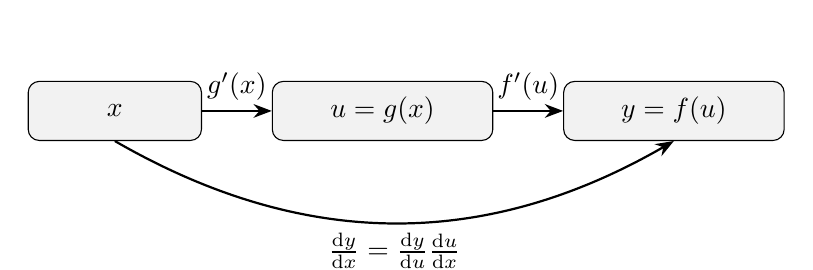
\begin{tikzpicture}[>=Stealth,scale=1.0]
  \node[draw,rounded corners,fill=gray!10,minimum width=2.2cm,minimum height=0.75cm] (x) at (0,0) {$x$};
  \node[draw,rounded corners,fill=gray!10,minimum width=2.8cm,minimum height=0.75cm] (u) at (3.4,0) {$u=g(x)$};
  \node[draw,rounded corners,fill=gray!10,minimum width=2.8cm,minimum height=0.75cm] (y) at (7.1,0) {$y=f(u)$};
  \draw[->,thick] (x) -- node[above] {$g'(x)$} (u);
  \draw[->,thick] (u) -- node[above] {$f'(u)$} (y);
  \draw[->,thick,bend right=30] (x.south) to node[below] {$\frac{\dd y}{\dd x}=\frac{\dd y}{\dd u}\frac{\dd u}{\dd x}$} (y.south);
\end{tikzpicture}
\end{center}

\begin{idea}
链式法则的关键是分清“外层函数”和“内层函数”. 若 $y=f(u)$、$u=g(x)$，则先对外层变量 $u$ 求导，再乘以内层对 $x$ 的导数. 多层复合时逐层相乘.
\end{idea}

\begin{example}[公式求导]
求 $y=(3x^2-1)^5$ 的导数.
\end{example}
\begin{solution}
令 $u=3x^2-1$，$y=u^5$. 由链式法则
\[
y'=5(3x^2-1)^4\cdot6x=30x(3x^2-1)^4.
\]
\end{solution}

\begin{example}[多层复合求导]
求
\[
y=\ee^{\sqrt{x}},\qquad x>0
\]
的导数.
\end{example}
\begin{solution}
这里有两层复合：
\[
x\longmapsto \sqrt{x}\longmapsto \ee^{\sqrt{x}}.
\]
因此
\[
y'=\ee^{\sqrt{x}}\cdot(\sqrt{x})'
=\ee^{\sqrt{x}}\cdot\frac{1}{2\sqrt{x}}
=\frac{\ee^{\sqrt{x}}}{2\sqrt{x}}.
\]
在 $x=0$ 处函数有定义，但上述导数公式不适用；事实上右差商趋于无穷大，因此在通常有限导数意义下不可导.
\end{solution}

\begin{example}[复合与乘积同时出现]
求
\[
y=\ee^{-x}\sin\sqrt{2x},\qquad x>0
\]
的导数.
\end{example}
\begin{solution}
这是两个函数的乘积，其中第二个函数又是复合函数. 由乘积法则，
\[
y'=(-\ee^{-x})\sin\sqrt{2x}
+\ee^{-x}\cdot\frac{\dd}{\dd x}\sin\sqrt{2x}.
\]
对第二项用链式法则：
\[
\frac{\dd}{\dd x}\sin\sqrt{2x}
=\cos\sqrt{2x}\cdot\frac{\dd}{\dd x}(2x)^{1/2}
=\cos\sqrt{2x}\cdot\frac1{\sqrt{2x}}.
\]
故
\[
y'=\ee^{-x}\left(\frac{\cos\sqrt{2x}}{\sqrt{2x}}-\sin\sqrt{2x}\right).
\]
\end{solution}

\begin{example}[对数求导]
求 $y=x^x\ (x>0)$ 的导数.
\end{example}
\begin{solution}
取对数得 $\ln y=x\ln x$. 两边求导：
\[
\frac{y'}{y}=\ln x+1.
\]
因此
\[
y'=x^x(\ln x+1).
\]
\end{solution}
\begin{warning}
$x^x$ 不能直接套用幂函数 $x^a$ 或指数函数 $a^x$ 的公式，因为底数和指数都含 $x$.
\end{warning}

\begin{example}[变底变指数函数]
求
\[
y=(\cot x)^{\cos x}
\]
的导数，其中在所讨论的区间内 $\cot x>0$.
\end{example}
\begin{solution}
由于底数和指数都含 $x$，采用对数求导. 取对数：
\[
\ln y=\cos x\ln(\cot x).
\]
两边对 $x$ 求导：
\[
\frac{y'}{y}
=-\sin x\ln(\cot x)+\cos x\cdot\frac{(\cot x)'}{\cot x}.
\]
又
\[
(\cot x)'=-\csc^2x,\qquad
\frac{(\cot x)'}{\cot x}
=-\frac{\csc^2x}{\cot x}
=-\frac{1}{\sin x\cos x}.
\]
于是
\[
\frac{y'}{y}
=-\sin x\ln(\cot x)-\frac1{\sin x}.
\]
因此
\[
y'=(\cot x)^{\cos x}\left[-\sin x\ln(\cot x)-\frac1{\sin x}\right].
\]
\end{solution}

\begin{example}[对数求导]
设
\[
y=\sqrt{\frac{(x-1)(x-2)}{(x-3)(x-4)}},
\]
其中 $x$ 取在使根式有意义且分母不为零的区间内. 求 $y'$.
\end{example}
\begin{solution}
取对数得
\[
\ln y=\frac12\left[\ln|x-1|+\ln|x-2|-\ln|x-3|-\ln|x-4|\right].
\]
两边求导：
\[
\frac{y'}{y}
=\frac12\left(\frac1{x-1}+\frac1{x-2}-\frac1{x-3}-\frac1{x-4}\right).
\]
因此
\[
y'=\frac12\sqrt{\frac{(x-1)(x-2)}{(x-3)(x-4)}}
\left(\frac1{x-1}+\frac1{x-2}-\frac1{x-3}-\frac1{x-4}\right).
\]
\end{solution}

\begin{proposition}[常用基本导数公式]
在相应定义域内，下列公式成立. 其中 $a>0,\ a\neq1$；对一般实数 $\alpha$，公式 $(x^\alpha)'=\alpha x^{\alpha-1}$ 通常在 $x>0$ 上使用，若 $\alpha$ 为整数或有理数，还需按函数本身的定义域作相应调整.
\[
(C)'=0,\quad (x^\alpha)'=\alpha x^{\alpha-1},\quad (a^x)'=a^x\ln a,\quad (\ee^x)'=\ee^x,
\]
\[
(\log_a |x|)'=\frac1{x\ln a},\quad (\ln |x|)'=\frac1x,
\]
\[
(\sin x)'=\cos x,\quad (\cos x)'=-\sin x,\quad
(\tan x)'=\sec^2x,\quad (\cot x)'=-\csc^2x,
\]
\[
(\sec x)'=\sec x\tan x,\quad (\csc x)'=-\csc x\cot x,
\]
\[
(\arcsin x)'=\frac1{\sqrt{1-x^2}},\quad
(\arccos x)'=-\frac1{\sqrt{1-x^2}},
\]
\[
(\arctan x)'=\frac1{1+x^2},\quad
(\operatorname{arccot}x)'=-\frac1{1+x^2}.
\]
\end{proposition}
\begin{idea}
这些公式是求导计算的基础. 讲授时不宜只背公式：三角函数公式来自导数定义与基本极限，指数与反三角函数公式分别依赖反函数求导和链式法则.
\end{idea}

\subsection{反函数求导与高阶导数}

有些函数本身不是由初等四则运算直接给出，而是作为另一个函数的反函数出现. 例如 $\ln x$ 是 $\ee^x$ 的反函数，$\arcsin x$ 是适当限制定义域后的 $\sin x$ 的反函数. 反函数求导公式说明：若 $y=f(x)$ 可反解为 $x=\varphi(y)$，则反函数图像在对应点的切线斜率等于原函数切线斜率的倒数.

\begin{theorem}[反函数求导公式]
设 $y=f(x)$ 在点 $x_0$ 的某邻域内严格单调、连续，且 $f$ 在 $x_0$ 处可导，$f'(x_0)\neq0$. 设反函数为 $x=\varphi(y)$，$y_0=f(x_0)$. 若 $\varphi$ 在 $y_0$ 处连续，则 $\varphi$ 在 $y_0$ 处可导，且
\[
\varphi'(y_0)=\frac{1}{f'(x_0)}.
\]
\end{theorem}
\begin{proofdetail}
当 $\Delta y\neq0$ 时，由严格单调性知对应的 $\Delta x=\varphi(y_0+\Delta y)-\varphi(y_0)$ 也不为 $0$，并且
\[
\frac{\Delta x}{\Delta y}
=\frac{1}{\frac{f(x_0+\Delta x)-f(x_0)}{\Delta x}}.
\]
由 $\varphi$ 在 $y_0$ 连续，$\Delta y\to0$ 时 $\Delta x\to0$. 因 $f'(x_0)\neq0$，
\[
\lim_{\Delta y\to0}\frac{\Delta x}{\Delta y}
=\frac{1}{\lim_{\Delta x\to0}\frac{f(x_0+\Delta x)-f(x_0)}{\Delta x}}
=\frac1{f'(x_0)}.
\]
故反函数在 $y_0$ 处可导，公式成立.
\end{proofdetail}

\begin{example}[由反函数推出对数函数导数]
由 $y=\log_a x\ (a>0,\ a\neq1,\ x>0)$，推出其导数公式.
\end{example}
\begin{solution}
令 $y=\log_a x$，则 $x=a^y$. 把 $x$ 看成 $y$ 的函数，有
\[
\frac{\dd x}{\dd y}=a^y\ln a=x\ln a.
\]
由反函数求导公式，
\[
\frac{\dd y}{\dd x}
=\frac{1}{\dd x/\dd y}
=\frac{1}{x\ln a}.
\]
当 $a=\ee$ 时得到
\[
(\ln x)'=\frac1x.
\]
\end{solution}

\begin{example}[反三角函数导数]
求 $y=\arcsin x$ 与 $y=\arctan x$ 的导数.
\end{example}
\begin{solution}
若 $y=\arcsin x$，则
\[
x=\sin y,\qquad y\in\left[-\frac{\pi}{2},\frac{\pi}{2}\right].
\]
在 $|x|<1$ 时，$\cos y>0$，故
\[
\frac{\dd x}{\dd y}=\cos y=\sqrt{1-\sin^2y}=\sqrt{1-x^2}.
\]
由反函数求导公式，
\[
(\arcsin x)'=\frac{1}{\sqrt{1-x^2}},\qquad |x|<1.
\]

若 $y=\arctan x$，则 $x=\tan y$，$y\in(-\pi/2,\pi/2)$. 因而
\[
\frac{\dd x}{\dd y}=\sec^2y=1+\tan^2y=1+x^2,
\]
所以
\[
(\arctan x)'=\frac1{1+x^2},\qquad x\in\RR.
\]
\end{solution}

\begin{definition}[高阶导数]
若 $f'$ 在区间上仍可导，则其导数称为 $f$ 的二阶导数，记作 $f''$ 或 $\frac{\dd^2y}{\dd x^2}$. 递推地，$f^{(n)}=(f^{(n-1)})'$ 称为 $n$ 阶导数.
\end{definition}

如果 $s(t)$ 表示直线运动位移，则 $s'(t)$ 是速度，$s''(t)$ 是加速度. 在经济学中，边际函数的导数也有意义：例如 $C''(x)$ 描述边际成本随产量变化的快慢. 因此高阶导数不仅是形式计算，也常用于判断变化趋势、凹凸性和近似公式.

\begin{example}[常用函数高阶导数]
求 $f(x)=\ee^{ax}$ 与 $g(x)=\sin x$ 的 $n$ 阶导数.
\end{example}
\begin{solution}
对指数函数，逐次求导得
\[
f^{(n)}(x)=a^n\ee^{ax}.
\]
对正弦函数，导数每四次循环：
\[
g^{(n)}(x)=\sin\left(x+\frac{n\pi}{2}\right).
\]
可用数学归纳法验证：$n=0$ 成立；若 $g^{(n)}(x)=\sin(x+n\pi/2)$，则
\[
g^{(n+1)}(x)=\cos\left(x+\frac{n\pi}{2}\right)=\sin\left(x+\frac{(n+1)\pi}{2}\right).
\]
\end{solution}

\begin{example}[对数函数的高阶导数]
求 $y=\ln(1+x)$ 的 $n$ 阶导数，其中 $x>-1$.
\end{example}
\begin{solution}
逐次求导：
\[
y'=\frac1{1+x},\qquad
y''=-\frac1{(1+x)^2},\qquad
y'''=\frac{2!}{(1+x)^3}.
\]
由此归纳得到
\[
y^{(n)}=(-1)^{n-1}\frac{(n-1)!}{(1+x)^n},\qquad n=1,2,3,\ldots.
\]
验证如下. 当 $n=1$ 时公式成立. 若
\[
y^{(n)}=(-1)^{n-1}(n-1)!(1+x)^{-n},
\]
则
\[
y^{(n+1)}
=(-1)^{n-1}(n-1)![-n(1+x)^{-n-1}]
=(-1)^n\frac{n!}{(1+x)^{n+1}}.
\]
故公式对所有正整数 $n$ 成立.
\end{solution}

\begin{example}[验证二阶导数关系]
设 $y=\ee^x\sin x$，证明
\[
y''-2y'+2y=0.
\]
\end{example}
\begin{solution}
先求一阶导数：
\[
y'=\ee^x\sin x+\ee^x\cos x=\ee^x(\sin x+\cos x).
\]
再求二阶导数：
\[
y''=\ee^x(\sin x+\cos x)+\ee^x(\cos x-\sin x)=2\ee^x\cos x.
\]
因此
\[
y''-2y'+2y
=2\ee^x\cos x-2\ee^x(\sin x+\cos x)+2\ee^x\sin x=0.
\]
等式成立.
\end{solution}

\begin{example}[Leibniz 公式]
求 $y=x^2\ee^x$ 的 $n$ 阶导数.
\end{example}
\begin{solution}
Leibniz 公式为
\[
(uv)^{(n)}=\sum_{k=0}^n\binom nk u^{(k)}v^{(n-k)}.
\]
取 $u=x^2,\ v=\ee^x$. 当 $k\geq3$ 时 $u^{(k)}=0$，故
\[
y^{(n)}=\binom n0x^2\ee^x+\binom n1(2x)\ee^x+\binom n2(2)\ee^x
=\ee^x\left[x^2+2nx+n(n-1)\right].
\]
\end{solution}

\begin{theorem}[Leibniz 公式]
若 $u,v$ 均有 $n$ 阶导数，则
\[
(uv)^{(n)}=\sum_{k=0}^{n}\binom{n}{k}u^{(k)}v^{(n-k)}.
\]
\end{theorem}
\begin{proofdetail}
用数学归纳法. 当 $n=1$ 时即乘法求导法则. 假设公式对 $n$ 成立，则
\[
(uv)^{(n+1)}
=\frac{\dd}{\dd x}\sum_{k=0}^{n}\binom{n}{k}u^{(k)}v^{(n-k)}
\]
\[
=\sum_{k=0}^{n}\binom{n}{k}u^{(k+1)}v^{(n-k)}
+\sum_{k=0}^{n}\binom{n}{k}u^{(k)}v^{(n-k+1)}.
\]
第一和中令 $j=k+1$，得
\[
\sum_{j=1}^{n+1}\binom{n}{j-1}u^{(j)}v^{(n+1-j)}
+\sum_{j=0}^{n}\binom{n}{j}u^{(j)}v^{(n+1-j)}.
\]
合并同类项，端点系数为 $1$，中间项系数为
\[
\binom{n}{j-1}+\binom{n}{j}=\binom{n+1}{j}.
\]
于是
\[
(uv)^{(n+1)}=\sum_{j=0}^{n+1}\binom{n+1}{j}u^{(j)}v^{(n+1-j)}.
\]
归纳完成.
\end{proofdetail}

\subsection{隐函数求导与参数方程求导}

前面讨论的函数大多写成 $y=f(x)$，这种形式称为显函数. 但在实际问题和几何问题中，变量之间常由方程给出，例如
\[
x^2+y^2=1,\qquad x^2+xy+y^2=3.
\]
它们未必能方便地解出 $y=f(x)$. 由方程 $F(x,y)=0$ 在某个范围内确定的函数称为隐函数. 例如
\[
\sqrt{y}+x^2-1=0
\]
在满足 $1-x^2\geq0$ 且 $\sqrt{y}=1-x^2$ 的范围内可写成
\[
y=(1-x^2)^2.
\]
但并不是每个方程都在任意点附近确定唯一函数. 本讲义在求导时默认题目所给方程已经在所讨论点附近确定了可导函数；更一般的存在唯一性条件将在多元函数课程中进一步解释.

\begin{center}
\begin{tikzpicture}[scale=1.15,>=Stealth]
  \draw[->] (-1.9,0) -- (1.9,0) node[right] {$x$};
  \draw[->] (0,-1.55) -- (0,1.55) node[above] {$y$};
  \draw[thick,domain=0:360,samples=160] plot ({cos(\x)},{sin(\x)});
  \fill (0.6,0.8) circle (1.5pt) node[above right] {$P(x,y)$};
  \draw[dashed] (0.6,0) -- (0.6,0.8) -- (0,0.8);
  \node at (0,-1.85) {$x^2+y^2=1$ 给出的曲线可在局部看作 $y=y(x)$};
\end{tikzpicture}
\end{center}

\begin{proposition}[隐函数一阶求导]
若方程 $F(x,y)=0$ 在某区间上确定可导函数 $y=y(x)$，且 $F$ 有连续偏导数、$F_y(x,y)\neq0$，则
\[
y'=-\frac{F_x}{F_y},
\]
其中右端在 $(x,y(x))$ 处取值.
\end{proposition}
\begin{proofdetail}
由恒等式 $F(x,y(x))\equiv0$ 对 $x$ 求导. 复合函数求导给出
\[
F_x(x,y(x))+F_y(x,y(x))y'(x)=0.
\]
由于 $F_y(x,y(x))\neq0$，移项并相除得到公式.
\end{proofdetail}

\begin{example}[隐函数一阶导数]
由方程 $x^2+xy+y^2=3$ 确定 $y=y(x)$，求 $y'$.
\end{example}
\begin{solution}
两边对 $x$ 求导：
\[
2x+y+xy'+2yy'=0.
\]
整理得
\[
y'=-\frac{2x+y}{x+2y}.
\]
该公式在 $x+2y\neq0$ 的点成立.
\end{solution}

\begin{example}[先说明隐函数再求导]
设方程
\[
\sqrt{y}+x^2-1=0
\]
在 $|x|<1$ 附近确定函数 $y=y(x)$. 用两种方法求 $y'$.
\end{example}
\begin{solution}
方法一：先解出显函数. 由方程得
\[
\sqrt{y}=1-x^2.
\]
当 $|x|<1$ 时右端为正，故
\[
y=(1-x^2)^2.
\]
于是
\[
y'=2(1-x^2)(-2x)=-4x(1-x^2).
\]

方法二：直接对原方程求导. 注意
\[
\frac{\dd}{\dd x}\sqrt{y}
=\frac{1}{2\sqrt{y}}y',
\]
因此
\[
\frac{y'}{2\sqrt{y}}+2x=0,
\qquad
y'=-4x\sqrt{y}.
\]
再代入 $\sqrt{y}=1-x^2$，得
\[
y'=-4x(1-x^2).
\]
两种方法结果一致.
\end{solution}

\begin{example}[隐函数二阶导数]
设 $x^2+y^2=1$ 在点附近确定 $y=y(x)$，求 $y''$.
\end{example}
\begin{solution}
一阶求导得
\[
2x+2yy'=0,\qquad y'=-\frac{x}{y}\quad(y\neq0).
\]
对 $2x+2yy'=0$ 再求导：
\[
2+2(y')^2+2yy''=0.
\]
故
\[
y''=-\frac{1+(y')^2}{y}=-\frac{1+x^2/y^2}{y}
=-\frac{x^2+y^2}{y^3}=-\frac1{y^3}.
\]
\end{solution}

\begin{example}[隐函数切线]
求曲线
\[
xy-\ee^x+\ee^y=0
\]
在点 $(0,0)$ 处的切线方程.
\end{example}
\begin{solution}
把 $y$ 看成 $x$ 的函数，对方程两边求导，得
\[
y+xy'-\ee^x+\ee^y y'=0.
\]
整理得
\[
(x+\ee^y)y'=\ee^x-y,\qquad
y'=\frac{\ee^x-y}{x+\ee^y}.
\]
在 $(0,0)$ 处，
\[
y'(0)=\frac{1-0}{0+1}=1.
\]
因此切线方程为 $y=x$.
\end{solution}

\begin{proposition}[参数方程求导]
若曲线由 $x=\varphi(t),\,y=\psi(t)$ 给出，且 $\varphi'(t)\neq0$，则
\[
\frac{\dd y}{\dd x}=\frac{\psi'(t)}{\varphi'(t)}.
\]
若还存在二阶导数，则
\[
\frac{\dd^2y}{\dd x^2}
=\frac{1}{\varphi'(t)}\frac{\dd}{\dd t}\left(\frac{\psi'(t)}{\varphi'(t)}\right).
\]
\end{proposition}
\begin{proofdetail}
当 $\varphi'(t)\neq0$ 时，局部可把 $t$ 看成 $x$ 的函数. 由链式法则，
\[
\frac{\dd y}{\dd t}=\frac{\dd y}{\dd x}\frac{\dd x}{\dd t}.
\]
两边除以 $\dd x/\dd t=\varphi'(t)$ 得第一式. 对第一式再关于 $x$ 求导，而 $\frac{\dd}{\dd x}=\frac1{\varphi'(t)}\frac{\dd}{\dd t}$，得第二式.
\end{proofdetail}

\begin{example}[参数方程求切线]
曲线由
\[
x=t^2,\qquad y=t^3
\]
给出. 求 $t=1$ 处的切线方程.
\end{example}
\begin{solution}
当 $t=1$ 时，曲线上的点为 $(1,1)$. 又
\[
\frac{\dd y}{\dd x}
=\frac{\dd y/\dd t}{\dd x/\dd t}
=\frac{3t^2}{2t}
=\frac{3t}{2}\qquad(t\neq0).
\]
在 $t=1$ 处斜率为 $3/2$，故切线方程为
\[
y-1=\frac32(x-1).
\]
\end{solution}

\begin{example}[增长率]
某种药物在血液中的浓度 $C$ 与时间 $t$ 的关系为 $C(t)=te^{-0.5t}$，求浓度变化率，并判断 $t=2$ 时浓度是增加还是减少.
\end{example}
\begin{solution}
\[
C'(t)=e^{-0.5t}-0.5te^{-0.5t}=e^{-0.5t}(1-0.5t).
\]
当 $t=2$ 时，$C'(2)=0$，说明此刻浓度达到由增转减的临界状态；仅从瞬时变化率看，此刻既不增加也不减少.
\end{solution}

\begin{example}[边际成本变化率]
某产品总成本函数为
\[
C(x)=0.02x^2+6x+300,\qquad x\geq0.
\]
求边际成本和边际成本的变化率，并解释 $C''(x)$ 的含义.
\end{example}
\begin{solution}
边际成本是总成本对产量的导数：
\[
C'(x)=0.04x+6.
\]
边际成本的变化率为
\[
C''(x)=0.04.
\]
这说明产量每增加一个单位，边际成本按近似 $0.04$ 的速度增加. 这里 $C'(x)$ 表示“在产量为 $x$ 附近多生产一个单位所增加的成本”，而 $C''(x)$ 描述这个边际成本本身随产量增加而上升的快慢.
\end{solution}

\subsection{课后习题}
\begin{enumerate}[label=\textbf{练习\arabic*.},leftmargin=2.2em]
\item 求下列函数的导数：
\[
y=3x^2+4\ln x-5\cos x,\qquad
y=\ln(\sin x),\qquad
y=\ee^{\sqrt{x}}.
\]
\item 求
\[
y=\frac{x^2\sin x}{1+x^2}
\]
的导数，并说明用到了哪些求导法则.
\item 求下列函数的导数：
\[
y=(1+x^2)^{\arctan x},\qquad
y=(\cot x)^{\cos x}.
\]
\item 由反函数求导公式推出 $y=\arccos x$ 的导数.
\item 求 $y=x^2\ln x$ 的二阶导数，其中 $x>0$.
\item 求 $y=x^2\ee^x$ 的 $n$ 阶导数.
\item 设 $x^3+y^3-3xy=0$ 确定 $y=y(x)$，求 $y'$.
\item 求曲线
\[
xy+\ln y=1
\]
在点 $(1,1)$ 处的切线方程.
\item 曲线由参数方程
\[
x=t-\sin t,\qquad y=1-\cos t
\]
给出，求 $\frac{\dd y}{\dd x}$.
\item 某产品总收入函数为
\[
R(x)=50x-0.1x^2.
\]
求边际收入函数和边际收入的变化率，并解释 $R''(x)$ 的经济含义.
\end{enumerate}

\subsection{参考解答}
\begin{enumerate}[label=\textbf{练习\arabic*.},leftmargin=2.2em]
\item
\[
(3x^2+4\ln x-5\cos x)'=6x+\frac4x+5\sin x.
\]
又
\[
(\ln\sin x)'=\frac{\cos x}{\sin x}=\cot x,
\]
其中需 $\sin x>0$ 或至少在选定区间内 $\ln(\sin x)$ 有定义. 最后
\[
(\ee^{\sqrt{x}})'=\ee^{\sqrt{x}}\cdot\frac1{2\sqrt{x}}
=\frac{\ee^{\sqrt{x}}}{2\sqrt{x}},\qquad x>0.
\]
\item 先对分子用乘积法则，再对整体用商法：
\[
\left(x^2\sin x\right)'=2x\sin x+x^2\cos x,
\]
\[
y'=\frac{(2x\sin x+x^2\cos x)(1+x^2)-2x\cdot x^2\sin x}{(1+x^2)^2}.
\]
化简得
\[
y'=\frac{2x\sin x+x^2\cos x+x^4\cos x}{(1+x^2)^2}.
\]
\item 对第一个函数取对数：
\[
\ln y=(\arctan x)\ln(1+x^2),
\]
故
\[
y'=(1+x^2)^{\arctan x}\left[\frac{\ln(1+x^2)}{1+x^2}+\frac{2x\arctan x}{1+x^2}\right].
\]
对第二个函数，取对数得
\[
\ln y=\cos x\ln(\cot x).
\]
因此
\[
y'=(\cot x)^{\cos x}\left[-\sin x\ln(\cot x)-\frac1{\sin x}\right],
\]
其中要求在所讨论区间内 $\cot x>0$.
\item 令 $y=\arccos x$，则 $x=\cos y$，$y\in[0,\pi]$. 当 $-1<x<1$ 时，$\sin y>0$，故
\[
\frac{\dd x}{\dd y}=-\sin y=-\sqrt{1-x^2}.
\]
由反函数求导公式，
\[
(\arccos x)'=-\frac1{\sqrt{1-x^2}},\qquad -1<x<1.
\]
\item
\[
y'=2x\ln x+x,\qquad y''=2\ln x+3.
\]
\item 由 Leibniz 公式，取 $u=x^2,\ v=\ee^x$. 因 $u^{(k)}=0\ (k\geq3)$，得
\[
y^{(n)}=\ee^x\left[x^2+2nx+n(n-1)\right].
\]
\item 两边对 $x$ 求导：
\[
3x^2+3y^2y'-3y-3xy'=0,
\]
故
\[
y'=\frac{y-x^2}{y^2-x}.
\]
\item 将 $y$ 看成 $x$ 的函数. 对
\[
xy+\ln y=1
\]
两边求导：
\[
y+xy'+\frac{y'}{y}=0.
\]
在 $(1,1)$ 处，
\[
1+y'+y'=0,\qquad y'=-\frac12.
\]
故切线方程为
\[
y-1=-\frac12(x-1).
\]
\item
\[
\frac{\dd y}{\dd x}=\frac{\sin t}{1-\cos t},
\]
其中 $1-\cos t\neq0$.
\item
\[
R'(x)=50-0.2x,\qquad R''(x)=-0.2.
\]
其中 $R'(x)$ 为边际收入，表示销量在 $x$ 附近增加一个单位时收入的近似增量；$R''(x)=-0.2$ 表示边际收入随销量增加而下降，且下降速度为常数 $0.2$.
\end{enumerate}

\section{微分与多元函数微分}
\renewEnvironmentCounter
\subsection{一元函数的微分与线性近似}

前两章中，导数描述的是函数在一点的瞬时变化率. 微分进一步强调另一件事：在自变量改变量很小时，函数增量的主要部分是一个线性函数. 这正是“用直线近似曲线”“用切平面近似曲面”的数学基础.

以正方形面积为例. 设边长为 $x$，面积为 $S=x^2$. 当边长由 $x$ 增加到 $x+\Delta x$，其中图中取 $\Delta x>0$，面积增量为
\[
\Delta S=(x+\Delta x)^2-x^2=2x\Delta x+(\Delta x)^2.
\]
这里 $2x\Delta x$ 是关于 $\Delta x$ 的线性主部，$(\Delta x)^2$ 是比 $\Delta x$ 高阶的误差项. 因而当 $|\Delta x|$ 很小时，
\[
\Delta S\approx 2x\Delta x.
\]

\begin{center}
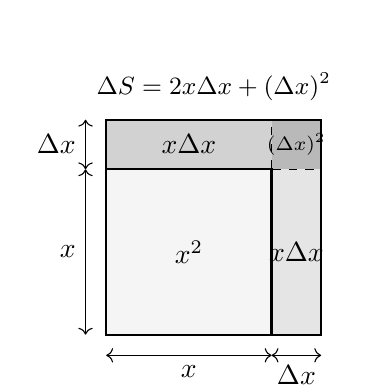
\begin{tikzpicture}[scale=1.05]
  \fill[gray!8] (0,0) rectangle (2,2);
  \fill[gray!20] (2,0) rectangle (2.6,2);
  \fill[gray!35] (0,2) rectangle (2,2.6);
  \fill[gray!55] (2,2) rectangle (2.6,2.6);
  \draw[thick] (0,0) rectangle (2,2);
  \draw[thick] (0,0) rectangle (2.6,2.6);
  \draw[dashed] (2,0)--(2,2.6);
  \draw[dashed] (0,2)--(2.6,2);
  \draw[<->] (0,-0.25)--(2,-0.25) node[midway,below] {$x$};
  \draw[<->] (2,-0.25)--(2.6,-0.25) node[midway,below] {$\Delta x$};
  \draw[<->] (-0.25,0)--(-0.25,2) node[midway,left] {$x$};
  \draw[<->] (-0.25,2)--(-0.25,2.6) node[midway,left] {$\Delta x$};
  \node at (1,1) {$x^2$};
  \node at (2.3,1) {$x\Delta x$};
  \node at (1,2.3) {$x\Delta x$};
  \node at (2.3,2.3) {\scriptsize $(\Delta x)^2$};
  \node at (1.3,3.0) {\small $\Delta S=2x\Delta x+(\Delta x)^2$};
\end{tikzpicture}
\end{center}

\begin{definition}[一元函数可微与微分]
设函数 $y=f(x)$ 在 $x$ 附近有定义. 当自变量增量为 $\Delta x$ 时，函数增量为
\[
\Delta y=f(x+\Delta x)-f(x).
\]
若存在与 $\Delta x$ 无关的常数 $A$，使得
\[
\Delta y=A\Delta x+o(\Delta x)\qquad(\Delta x\to0),
\]
则称 $f$ 在 $x$ 处可微，并称线性主部 $A\Delta x$ 为 $f$ 在 $x$ 处的微分，记作
\[
\dd y=A\Delta x.
\]
通常记 $\dd x=\Delta x$，于是微分写成 $\dd y=A\dd x$.
\end{definition}

\begin{theorem}[一元可导与可微等价]
$f$ 在 $x$ 处可微，当且仅当 $f$ 在 $x$ 处可导. 此时
\[
A=f'(x),\qquad \dd y=f'(x)\dd x.
\]
\end{theorem}
\begin{proofdetail}
若 $f$ 在 $x$ 处可微，则
\[
f(x+\Delta x)-f(x)=A\Delta x+o(\Delta x).
\]
当 $\Delta x\neq0$ 时，两边除以 $\Delta x$，得
\[
\frac{f(x+\Delta x)-f(x)}{\Delta x}
=A+\frac{o(\Delta x)}{\Delta x}.
\]
由 $o(\Delta x)$ 的定义，
\[
\frac{o(\Delta x)}{\Delta x}\to0\qquad(\Delta x\to0),
\]
所以导数存在，且 $f'(x)=A$.

反过来，若 $f$ 在 $x$ 处可导，则
\[
\frac{f(x+\Delta x)-f(x)}{\Delta x}\to f'(x).
\]
定义
\[
\alpha(\Delta x)=
\begin{cases}
\dfrac{f(x+\Delta x)-f(x)}{\Delta x}-f'(x),&\Delta x\neq0,\\[0.8em]
0,&\Delta x=0.
\end{cases}
\]
则 $\alpha(\Delta x)\to0$，并且
\[
\Delta y=f'(x)\Delta x+\alpha(\Delta x)\Delta x
=f'(x)\Delta x+o(\Delta x).
\]
因此 $f$ 在 $x$ 处可微，且 $\dd y=f'(x)\dd x$.
\end{proofdetail}

\begin{proposition}[微分运算法则]
若 $u=u(x),v=v(x)$ 在 $x$ 处可微，$c$ 为常数，则
\[
\dd(cu)=c\,\dd u,\qquad \dd(u+v)=\dd u+\dd v,
\]
\[
\dd(uv)=u\,\dd v+v\,\dd u,
\]
若 $v\neq0$，则
\[
\dd\left(\frac{u}{v}\right)=\frac{v\,\dd u-u\,\dd v}{v^2}.
\]
若 $y=f(u)$，$u=g(x)$，且相应函数可微，则
\[
\dd y=f'(u)\dd u.
\]
\end{proposition}
\begin{proofdetail}
由一元可导与可微等价，$u,v$ 可微等价于可导. 前四个公式分别由常数倍、和、积、商的求导法则乘以 $\dd x$ 得到. 例如
\[
\dd(uv)=(uv)'\dd x=(u'v+uv')\dd x=v(u'\dd x)+u(v'\dd x)=v\,\dd u+u\,\dd v.
\]
复合情形中，链式法则给出
\[
\dd y=\frac{\dd y}{\dd x}\dd x=f'(u)g'(x)\dd x=f'(u)\dd u.
\]
这说明无论 $u$ 是自变量还是 $x$ 的函数，微分形式 $\dd y=f'(u)\dd u$ 保持不变.
\end{proofdetail}

\begin{proposition}[微分的几何意义]
若 $f$ 在 $x_0$ 处可导，则曲线 $y=f(x)$ 在点 $M=(x_0,f(x_0))$ 附近可用切线作局部近似：
\[
f(x_0+\Delta x)-f(x_0)=f'(x_0)\Delta x+o(\Delta x).
\]
其中 $\Delta y=f(x_0+\Delta x)-f(x_0)$ 是真实增量，$\dd y=f'(x_0)\Delta x$ 是切线给出的线性近似，二者差为高阶误差.
\end{proposition}

\begin{center}
\begin{tikzpicture}[scale=1.0,>=Stealth]
  \draw[->] (-0.2,0)--(6.4,0) node[right] {$x$};
  \draw[->] (0,0.35)--(0,3.1) node[above] {$y$};
  \draw[domain=0.55:4.9,smooth,variable=\x,thick] plot ({\x},{0.16*(\x-1)*(\x-1)+1});
  \coordinate (M) at (2,1.16);
  \coordinate (T) at (3.4,1.608);
  \coordinate (N) at (3.4,1.922);
  \coordinate (B) at (3.4,1.16);
  \draw[thick] (0.7,0.744)--(5.15,2.168);
  \draw[dashed] (M)--(2,0) node[below] {$x_0$};
  \draw[dashed] (N)--(3.4,0) node[below] {$x_0+\Delta x$};
  \draw[dashed] (M)--(B);
  \draw[dashed] (N)--(T);
  \draw[dashed] (T)--(B);
  \draw[<->] (2,0.55)--(3.4,0.55) node[midway,below] {$\Delta x$};
  \draw[<->] (3.66,1.16)--(3.66,1.608);
  \draw[<->] (3.66,1.608)--(3.66,1.922);
  \draw[thin] (3.66,1.384)--(4.65,1.34) node[right] {$\dd y$};
  \draw[thin] (3.66,1.765)--(4.65,1.78) node[right] {\scriptsize $\Delta y-\dd y$};
  \fill (M) circle (1.5pt) node[above left] {$M$};
  \fill (T) circle (1.4pt) node[below left] {$T$};
  \fill (N) circle (1.5pt) node[above left] {$N$};
  \node[fill=white,inner sep=1pt] at (4.95,2.35) {切线};
\end{tikzpicture}
\end{center}

\begin{example}[近似计算]
用微分近似计算 $\sqrt{4.04}$.
\end{example}
\begin{solution}
取 $f(x)=\sqrt{x}$，在 $x=4$ 处线性化. 有
\[
f(4)=2,\qquad f'(x)=\frac{1}{2\sqrt{x}},\qquad f'(4)=\frac14.
\]
当 $\Delta x=0.04$ 时，
\[
\sqrt{4.04}=f(4+0.04)\approx f(4)+f'(4)\Delta x
=2+\frac14\cdot0.04=2.01.
\]
\end{solution}
\begin{warning}
微分近似不是等式. 本题真实值约为 $2.009975\cdots$，近似值 $2.01$ 的误差很小，是因为 $\Delta x=0.04$ 相对基点 $4$ 很小.
\end{warning}

\begin{example}[相对误差]
球的半径 $r$ 测量有小误差 $\Delta r$. 设体积 $V=\frac43\pi r^3$. 用微分估计体积的相对误差.
\end{example}
\begin{solution}
体积微分为
\[
\dd V=4\pi r^2\dd r.
\]
当 $\Delta r$ 很小时，$\Delta V\approx \dd V=4\pi r^2\Delta r$. 因此体积相对误差近似为
\[
\frac{\Delta V}{V}\approx
\frac{\dd V}{V}
=\frac{4\pi r^2\dd r}{\frac43\pi r^3}
=3\frac{\dd r}{r}.
\]
这说明半径的相对误差约放大为体积相对误差的三倍. 该结论来自数学模型 $V=\frac43\pi r^3$，不依赖具体计量单位.
\end{solution}

\begin{example}[微分形式不变性]
求函数
\[
y=\ee^{1-3x}\sin2x
\]
的微分.
\end{example}
\begin{solution}
由乘积微分法则，
\[
\dd y=\sin2x\,\dd(\ee^{1-3x})+\ee^{1-3x}\,\dd(\sin2x).
\]
利用微分形式不变性，
\[
\dd(\ee^{1-3x})=\ee^{1-3x}\dd(1-3x)=-3\ee^{1-3x}\dd x,
\]
\[
\dd(\sin2x)=\cos2x\,\dd(2x)=2\cos2x\,\dd x.
\]
故
\[
\dd y=\ee^{1-3x}(2\cos2x-3\sin2x)\dd x.
\]
\end{solution}

\subsection{偏导数与高阶偏导数}

二元函数 $z=f(x,y)$ 的输入是平面上的点. 若只让 $x$ 改变而保持 $y$ 不变，就得到沿平行于 $x$ 轴方向的变化率；若只让 $y$ 改变而保持 $x$ 不变，就得到沿平行于 $y$ 轴方向的变化率. 这两个变化率分别称为偏导数.

\begin{definition}[偏导数]
设 $z=f(x,y)$ 在点 $(x_0,y_0)$ 的某邻域内有定义. 若极限
\[
\lim_{h\to0}\frac{f(x_0+h,y_0)-f(x_0,y_0)}{h}
\]
存在，则称其为 $f$ 对 $x$ 的偏导数，记为
\[
f_x(x_0,y_0),\qquad \frac{\partial f}{\partial x}(x_0,y_0).
\]
若极限
\[
\lim_{k\to0}\frac{f(x_0,y_0+k)-f(x_0,y_0)}{k}
\]
存在，则称其为 $f$ 对 $y$ 的偏导数，记为 $f_y(x_0,y_0)$ 或 $\frac{\partial f}{\partial y}(x_0,y_0)$.
\end{definition}

\begin{example}[偏导计算]
设 $f(x,y)=x^2y+\sin(xy)$，求 $f_x,f_y$.
\end{example}
\begin{solution}
求 $f_x$ 时把 $y$ 看作常数：
\[
f_x=2xy+y\cos(xy).
\]
求 $f_y$ 时把 $x$ 看作常数：
\[
f_y=x^2+x\cos(xy).
\]
偏导计算中的“把另一个变量看作常数”不是说另一个变量永远不变，而是说此刻只沿一个坐标方向取变化率.
\end{solution}

\begin{example}[边际产量]
设 Cobb-Douglas 型生产函数为
\[
Q(K,L)=A K^\alpha L^\beta,\qquad A>0,\quad K>0,\quad L>0.
\]
其中 $K$ 表示资本投入，$L$ 表示劳动投入，$Q$ 表示产出. 求资本的边际产量和劳动的边际产量.
\end{example}
\begin{solution}
资本的边际产量指在劳动投入 $L$ 固定时，产出对资本投入 $K$ 的偏导数：
\[
Q_K=A\alpha K^{\alpha-1}L^\beta.
\]
劳动的边际产量指在资本投入 $K$ 固定时，产出对劳动投入 $L$ 的偏导数：
\[
Q_L=A\beta K^\alpha L^{\beta-1}.
\]
这两个量分别表示在当前投入水平附近，单独增加一单位资本或一单位劳动时，产出的近似增量.
\end{solution}

\begin{definition}[二阶偏导数]
若一阶偏导函数 $f_x,f_y$ 仍有偏导数，则称这些偏导数为二阶偏导数，记作
\[
f_{xx}=\frac{\partial^2 f}{\partial x^2},\qquad
f_{xy}=\frac{\partial^2 f}{\partial y\partial x},
\]
\[
f_{yx}=\frac{\partial^2 f}{\partial x\partial y},\qquad
f_{yy}=\frac{\partial^2 f}{\partial y^2}.
\]
这里 $f_{xy}$ 表示先对 $x$ 求偏导，再对 $y$ 求偏导；$f_{yx}$ 表示先对 $y$ 求偏导，再对 $x$ 求偏导.
\end{definition}

\begin{theorem}[混合偏导相等的充分条件]
若 $f_{xy}$ 与 $f_{yx}$ 在点 $(x_0,y_0)$ 的某邻域内存在，并且都在 $(x_0,y_0)$ 连续，则
\[
f_{xy}(x_0,y_0)=f_{yx}(x_0,y_0).
\]
\end{theorem}
\begin{proofdetail}
取充分小的非零 $h,k$，记
\[
\Delta=f(x_0+h,y_0+k)-f(x_0+h,y_0)-f(x_0,y_0+k)+f(x_0,y_0).
\]
先把 $\Delta$ 写为
\[
\Delta=\bigl[f(x_0+h,y_0+k)-f(x_0,y_0+k)\bigr]
-\bigl[f(x_0+h,y_0)-f(x_0,y_0)\bigr].
\]
对函数
\[
\Phi(y)=f(x_0+h,y)-f(x_0,y)
\]
在区间端点 $y_0,y_0+k$ 使用一元中值定理，存在 $\eta$ 介于 $0$ 与 $k$ 之间，使
\[
\Delta=\Phi'(y_0+\eta)k
=\bigl[f_y(x_0+h,y_0+\eta)-f_y(x_0,y_0+\eta)\bigr]k.
\]
再对函数 $x\mapsto f_y(x,y_0+\eta)$ 在 $x_0,x_0+h$ 上使用中值定理，存在 $\xi$ 介于 $0$ 与 $h$ 之间，使
\[
\Delta=f_{yx}(x_0+\xi,y_0+\eta)hk.
\]
因此
\[
\frac{\Delta}{hk}=f_{yx}(x_0+\xi,y_0+\eta).
\]

另一方面，把 $\Delta$ 写为
\[
\Delta=\bigl[f(x_0+h,y_0+k)-f(x_0+h,y_0)\bigr]
-\bigl[f(x_0,y_0+k)-f(x_0,y_0)\bigr],
\]
同理可得存在 $\xi_1$ 介于 $0$ 与 $h$ 之间、$\eta_1$ 介于 $0$ 与 $k$ 之间，使
\[
\frac{\Delta}{hk}=f_{xy}(x_0+\xi_1,y_0+\eta_1).
\]
令 $(h,k)\to(0,0)$，由 $f_{xy},f_{yx}$ 在 $(x_0,y_0)$ 连续，两种表示的极限分别为 $f_{xy}(x_0,y_0)$ 与 $f_{yx}(x_0,y_0)$，而左端是同一个量的极限，故两者相等.
\end{proofdetail}

\begin{example}[二阶偏导]
设 $f(x,y)=x^3y^2+\ee^{xy}$，求 $f_{xy}$ 与 $f_{yx}$.
\end{example}
\begin{solution}
先求
\[
f_x=3x^2y^2+y\ee^{xy},
\]
再对 $y$ 求偏导：
\[
f_{xy}=6x^2y+\ee^{xy}+xy\ee^{xy}.
\]
另一方面，
\[
f_y=2x^3y+x\ee^{xy},
\]
再对 $x$ 求偏导：
\[
f_{yx}=6x^2y+\ee^{xy}+xy\ee^{xy}.
\]
两者相等. 这里函数由初等函数复合而成，各相关偏导连续，因此符合混合偏导相等的充分条件.
\end{solution}

\begin{example}[偏导存在不推出连续]
设
\[
f(x,y)=
\begin{cases}
\dfrac{xy}{x^2+y^2},&(x,y)\neq(0,0),\\[0.6em]
0,&(x,y)=(0,0).
\end{cases}
\]
证明 $f_x(0,0),f_y(0,0)$ 存在，但 $f$ 在 $(0,0)$ 不连续.
\end{example}
\begin{solution}
按定义，
\[
f_x(0,0)=\lim_{h\to0}\frac{f(h,0)-f(0,0)}{h}=0,\qquad
f_y(0,0)=\lim_{h\to0}\frac{f(0,h)-f(0,0)}{h}=0.
\]
但沿直线 $y=x$，
\[
f(x,x)=\frac{x^2}{2x^2}=\frac12\quad(x\neq0),
\]
故 $\lim_{(x,y)\to(0,0)}f(x,y)$ 不等于 $0$，函数在原点不连续.
\end{solution}
\begin{warning}
偏导数只检测坐标轴方向的变化，不能控制所有趋近方向. 因此“两个偏导数都存在”远弱于“一元函数可导”.
\end{warning}

\subsection{全微分与多元链式法则}

二元函数的偏导数只给出两个坐标方向的变化率. 若要像一元函数那样用一个线性表达式近似总增量，就需要全微分. 全微分的线性主部同时包含 $\Delta x$ 与 $\Delta y$：
\[
\Delta z\approx f_x(x_0,y_0)\Delta x+f_y(x_0,y_0)\Delta y.
\]

\begin{definition}[二元函数可微与全微分]
设 $z=f(x,y)$ 在 $(x_0,y_0)$ 附近有定义. 若
\[
\Delta z=f(x_0+\Delta x,y_0+\Delta y)-f(x_0,y_0)
\]
可写成
\[
\Delta z=A\Delta x+B\Delta y+o(\rho),
\qquad \rho=\sqrt{(\Delta x)^2+(\Delta y)^2},
\]
则称 $f$ 在 $(x_0,y_0)$ 可微，并称
\[
\dd z=A\dd x+B\dd y
\]
为 $f$ 在该点的全微分.
\end{definition}

\begin{theorem}[可微推出连续且偏导存在]
若 $f$ 在 $(x_0,y_0)$ 可微，则 $f$ 在该点连续，且 $f_x(x_0,y_0),f_y(x_0,y_0)$ 存在，并且
\[
\dd z=f_x(x_0,y_0)\dd x+f_y(x_0,y_0)\dd y.
\]
\end{theorem}
\begin{proofdetail}
由可微性，
\[
\Delta z=A\Delta x+B\Delta y+o(\rho).
\]
由于 $|\Delta x|\leq\rho,\ |\Delta y|\leq\rho$，当 $\rho\to0$ 时，
\[
A\Delta x+B\Delta y\to0,\qquad o(\rho)\to0.
\]
故 $\Delta z\to0$，即 $f$ 在 $(x_0,y_0)$ 连续.

取 $\Delta y=0$，则 $\rho=|\Delta x|$，且
\[
f(x_0+\Delta x,y_0)-f(x_0,y_0)=A\Delta x+o(|\Delta x|).
\]
当 $\Delta x\neq0$ 时除以 $\Delta x$ 并令 $\Delta x\to0$，得
\[
f_x(x_0,y_0)=A.
\]
同理取 $\Delta x=0$ 得 $f_y(x_0,y_0)=B$. 因此
\[
\dd z=f_x(x_0,y_0)\dd x+f_y(x_0,y_0)\dd y.
\]
\end{proofdetail}

\begin{theorem}[偏导连续推出可微]
若 $f_x,f_y$ 在 $(x_0,y_0)$ 的某邻域内存在，并且在 $(x_0,y_0)$ 连续，则 $f$ 在 $(x_0,y_0)$ 可微.
\end{theorem}
\begin{proofdetail}
记
\[
\Delta z=f(x_0+\Delta x,y_0+\Delta y)-f(x_0,y_0).
\]
分两段改变变量：
\[
\Delta z=[f(x_0+\Delta x,y_0+\Delta y)-f(x_0,y_0+\Delta y)]
+[f(x_0,y_0+\Delta y)-f(x_0,y_0)].
\]
对第一项把 $y_0+\Delta y$ 固定，对一元函数 $x\mapsto f(x,y_0+\Delta y)$ 使用中值定理. 当 $\Delta x\neq0$ 时，存在 $\theta_1\in(0,1)$ 使
\[
f(x_0+\Delta x,y_0+\Delta y)-f(x_0,y_0+\Delta y)
=f_x(x_0+\theta_1\Delta x,y_0+\Delta y)\Delta x.
\]
当 $\Delta x=0$ 时该等式也成立，因为两边均为 $0$，$\theta_1$ 可任取. 对第二项同理，存在 $\theta_2\in(0,1)$ 使
\[
f(x_0,y_0+\Delta y)-f(x_0,y_0)
=f_y(x_0,y_0+\theta_2\Delta y)\Delta y.
\]
于是
\[
\Delta z=f_x(x_0,y_0)\Delta x+f_y(x_0,y_0)\Delta y+R,
\]
其中
\[
R=[f_x(x_0+\theta_1\Delta x,y_0+\Delta y)-f_x(x_0,y_0)]\Delta x
\]
\[
\quad+[f_y(x_0,y_0+\theta_2\Delta y)-f_y(x_0,y_0)]\Delta y.
\]
由 $f_x,f_y$ 在 $(x_0,y_0)$ 连续，两个方括号中的差都趋于 $0$. 又 $|\Delta x|\leq\rho,\ |\Delta y|\leq\rho$，所以 $R=o(\rho)$. 因此 $f$ 可微.
\end{proofdetail}

\begin{center}
\begin{tikzpicture}[scale=1.0,>=Stealth]
  \draw[->] (-0.2,0)--(5.2,0) node[right] {$x$};
  \draw[->] (0,-0.2)--(0,3.4) node[above] {$y$};
  \coordinate (P) at (1.3,1.0);
  \coordinate (A) at (4.2,1.0);
  \coordinate (B) at (4.2,2.75);
  \coordinate (C) at (1.3,2.75);
  \draw[dashed] (P)--(A)--(B);
  \draw[dashed] (P)--(C)--(B);
  \draw[->,thick] (P)--(A) node[midway,below] {$\Delta x$};
  \draw[->,thick] (A)--(B) node[midway,right] {$\Delta y$};
  \draw[->,thick] (P)--(C) node[midway,left] {$\Delta y$};
  \draw[->,thick] (C)--(B) node[midway,above] {$\Delta x$};
  \fill (P) circle (1.5pt) node[below left] {$(x_0,y_0)$};
  \fill (B) circle (1.5pt) node[above right] {$(x_0+\Delta x,y_0+\Delta y)$};
  \node at (2.75,3.15) {\small 总增量可沿两段坐标方向分解};
\end{tikzpicture}
\end{center}

\begin{example}[全微分近似]
估计 $f(x,y)=x^2y+\ln y$ 在 $(2,1)$ 附近，当 $x$ 增加 $0.01$、$y$ 减少 $0.02$ 时的函数增量.
\end{example}
\begin{solution}
\[
f_x=2xy,\qquad f_y=x^2+\frac1y.
\]
在 $(2,1)$ 处，
\[
f_x(2,1)=4,\qquad f_y(2,1)=5.
\]
故
\[
\Delta f\approx \dd f=4(0.01)+5(-0.02)=0.04-0.10=-0.06.
\]
这里的 $-0.06$ 是函数真实增量的线性近似；若要得到真实增量，需要代入原函数计算.
\end{solution}

\begin{example}[可微性判断]
证明函数
\[
f(x,y)=x^2+y^2+xy
\]
在任意点可微，并求其全微分.
\end{example}
\begin{solution}
先求偏导数：
\[
f_x=2x+y,\qquad f_y=2y+x.
\]
这两个偏导函数在全平面连续. 由偏导连续推出可微的定理，$f$ 在任意点可微，且
\[
\dd z=(2x+y)\dd x+(2y+x)\dd y.
\]
\end{solution}

\begin{theorem}[二元链式法则：一元参数情形]
设 $z=f(x,y)$ 在点 $(x(t),y(t))$ 处可微，且 $x=x(t),y=y(t)$ 在 $t$ 处可导，则复合函数 $z=f(x(t),y(t))$ 在 $t$ 处可导，且
\[
\frac{\dd z}{\dd t}=f_x\frac{\dd x}{\dd t}+f_y\frac{\dd y}{\dd t},
\]
其中 $f_x,f_y$ 在点 $(x(t),y(t))$ 处取值.
\end{theorem}
\begin{proofdetail}
由 $f$ 可微，
\[
\Delta z=f_x\Delta x+f_y\Delta y+o(\rho),
\qquad \rho=\sqrt{(\Delta x)^2+(\Delta y)^2}.
\]
两边除以 $\Delta t$. 因 $x,y$ 在 $t$ 处可导，故
\[
\Delta x=x'(t)\Delta t+o(\Delta t),\qquad
\Delta y=y'(t)\Delta t+o(\Delta t).
\]
于是 $\rho=O(|\Delta t|)$. 因此
\[
\frac{o(\rho)}{\Delta t}
=\frac{o(\rho)}{\rho}\cdot\frac{\rho}{\Delta t}\to0,
\]
其中第二个因子有界. 令 $\Delta t\to0$，得到
\[
\frac{\dd z}{\dd t}=f_x x'(t)+f_y y'(t).
\]
\end{proofdetail}

\begin{center}
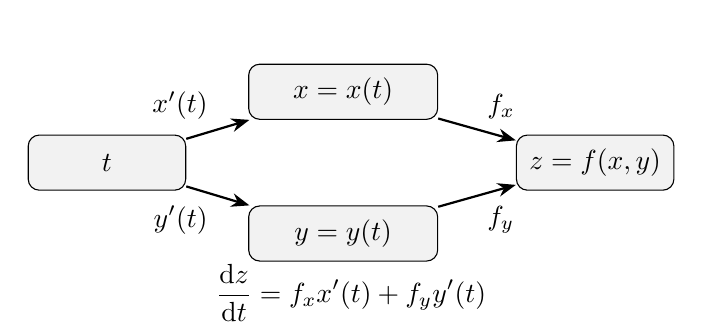
\begin{tikzpicture}[>=Stealth,scale=1.0]
  \node[draw,rounded corners,fill=gray!10,minimum width=2cm,minimum height=0.7cm] (t) at (0,0) {$t$};
  \node[draw,rounded corners,fill=gray!10,minimum width=2.4cm,minimum height=0.7cm] (x) at (3,0.9) {$x=x(t)$};
  \node[draw,rounded corners,fill=gray!10,minimum width=2.4cm,minimum height=0.7cm] (y) at (3,-0.9) {$y=y(t)$};
  \node[draw,rounded corners,fill=gray!10,minimum width=2cm,minimum height=0.7cm] (z) at (6.2,0) {$z=f(x,y)$};
  \draw[->,thick] (t)--(x) node[midway,above left] {$x'(t)$};
  \draw[->,thick] (t)--(y) node[midway,below left] {$y'(t)$};
  \draw[->,thick] (x)--(z) node[midway,above right] {$f_x$};
  \draw[->,thick] (y)--(z) node[midway,below right] {$f_y$};
  \node at (3.1,-1.65) {$\displaystyle \frac{\dd z}{\dd t}=f_xx'(t)+f_yy'(t)$};
\end{tikzpicture}
\end{center}

\begin{example}[多元链式法则]
设
\[
z=x^2y+\sin y,\qquad x=t^2,\qquad y=\ee^t.
\]
求 $\frac{\dd z}{\dd t}$.
\end{example}
\begin{solution}
先求
\[
z_x=2xy,\qquad z_y=x^2+\cos y.
\]
又
\[
\frac{\dd x}{\dd t}=2t,\qquad \frac{\dd y}{\dd t}=\ee^t.
\]
由链式法则，
\[
\frac{\dd z}{\dd t}
=z_x\frac{\dd x}{\dd t}+z_y\frac{\dd y}{\dd t}
=2xy\cdot2t+(x^2+\cos y)\ee^t.
\]
代入 $x=t^2,\ y=\ee^t$，得
\[
\frac{\dd z}{\dd t}
=4t^3\ee^t+(t^4+\cos(\ee^t))\ee^t.
\]
\end{solution}

\begin{theorem}[二元链式法则：二元中间变量情形]
设 $z=f(u,v)$ 在相应点可微，且
\[
u=u(x,y),\qquad v=v(x,y)
\]
在 $(x,y)$ 处有连续偏导数，则复合函数 $z=f(u(x,y),v(x,y))$ 在该点的偏导数为
\[
\frac{\partial z}{\partial x}=f_u\frac{\partial u}{\partial x}+f_v\frac{\partial v}{\partial x},
\qquad
\frac{\partial z}{\partial y}=f_u\frac{\partial u}{\partial y}+f_v\frac{\partial v}{\partial y}.
\]
\end{theorem}
\begin{proofdetail}
只证关于 $x$ 的公式，关于 $y$ 的公式同理. 固定 $y$，令 $x$ 改变为 $x+\Delta x$. 由于 $u,v$ 对 $x$ 可导，
\[
\Delta u=u_x\Delta x+o(\Delta x),\qquad
\Delta v=v_x\Delta x+o(\Delta x).
\]
由 $f$ 在 $(u,v)$ 处可微，
\[
\Delta z=f_u\Delta u+f_v\Delta v+o(\rho),
\qquad \rho=\sqrt{(\Delta u)^2+(\Delta v)^2}.
\]
又 $\Delta u=O(\Delta x),\Delta v=O(\Delta x)$，故 $\rho=O(|\Delta x|)$，从而 $o(\rho)=o(\Delta x)$. 代入得
\[
\Delta z=(f_u u_x+f_v v_x)\Delta x+o(\Delta x).
\]
两边除以 $\Delta x$ 并令 $\Delta x\to0$，得到
\[
\frac{\partial z}{\partial x}=f_u u_x+f_v v_x.
\]
\end{proofdetail}

\begin{example}[二元复合函数偏导]
设 $z=f(x^2+y,xy)$，其中 $f$ 有连续一阶偏导数. 求 $\frac{\partial z}{\partial x}$ 与 $\frac{\partial z}{\partial y}$.
\end{example}
\begin{solution}
令
\[
u=x^2+y,\qquad v=xy.
\]
则 $z=f(u,v)$. 记 $f_u,f_v$ 分别为 $f$ 对第一、第二个变量的偏导数，并在 $(u,v)=(x^2+y,xy)$ 处取值. 由链式法则，
\[
\frac{\partial z}{\partial x}
=f_u\frac{\partial u}{\partial x}+f_v\frac{\partial v}{\partial x}
=2x f_u+y f_v,
\]
\[
\frac{\partial z}{\partial y}
=f_u\frac{\partial u}{\partial y}+f_v\frac{\partial v}{\partial y}
=f_u+x f_v.
\]
\end{solution}

\subsection{课后习题}
\begin{enumerate}[label=\textbf{练习\arabic*.},leftmargin=2.2em]
\item 判断下列命题真伪，并说明理由：偏导数存在必连续；连续且偏导存在必可微；偏导数连续必可微；可微必连续.
\item 求 $z=x^2y+\ee^{xy}$ 的全微分.
\item 用微分近似计算 $\sqrt{9.06}$.
\item 用微分估计 $\ln(1.02)$.
\item 设 $f(x,y)=x^3y^2+\ee^{xy}$，求 $f_x,f_y,f_{xy},f_{yx}$.
\item 设生产函数 $Q(K,L)=10K^{1/2}L^{1/2}$. 求 $Q_K,Q_L$，并解释它们的意义.
\item 证明函数 $f(x,y)=x^2+y^2-2xy$ 在任意点可微，并写出全微分.
\item 设 $z=x^2y+\sin y,\ x=t^2,\ y=\ee^t$. 求 $\frac{\dd z}{\dd t}$.
\item 设 $z=f(x^2+y,xy)$，其中 $f$ 有连续一阶偏导数. 求 $\frac{\partial z}{\partial x}$ 与 $\frac{\partial z}{\partial y}$.
\item 设
\[
f(x,y)=
\begin{cases}
\dfrac{x^2y}{x^2+y^2},&(x,y)\neq(0,0),\\[0.6em]
0,&(x,y)=(0,0).
\end{cases}
\]
求 $f_x(0,0),f_y(0,0)$，并判断 $f$ 在 $(0,0)$ 是否连续.
\end{enumerate}

\subsection{参考解答}
\begin{enumerate}[label=\textbf{练习\arabic*.},leftmargin=2.2em]
\item 偏导数存在不一定连续，反例可取本章例题
\[
f(x,y)=\frac{xy}{x^2+y^2},\quad f(0,0)=0.
\]
连续且偏导存在不一定可微；例如
\[
f(x,y)=
\begin{cases}
\dfrac{xy}{\sqrt{x^2+y^2}},&(x,y)\neq(0,0),\\[0.6em]
0,&(x,y)=(0,0).
\end{cases}
\]
在原点连续，且
\[
f_x(0,0)=\lim_{h\to0}\frac{f(h,0)-0}{h}=0,\qquad
f_y(0,0)=\lim_{k\to0}\frac{f(0,k)-0}{k}=0.
\]
若它在原点可微，则线性主部应为 $0\cdot x+0\cdot y=0$. 但沿 $y=x$，
\[
\frac{f(x,x)-0}{\sqrt{x^2+x^2}}
=\frac{x^2/\sqrt{2x^2}}{\sqrt{2x^2}}
=\frac12\qquad(x\neq0),
\]
不趋于 $0$，故不可微. 偏导数在邻域内存在且在该点连续可推出可微；可微必连续.
\item
\[
z_x=2xy+y\ee^{xy},\qquad z_y=x^2+x\ee^{xy},
\]
所以
\[
\dd z=(2xy+y\ee^{xy})\dd x+(x^2+x\ee^{xy})\dd y.
\]
\item 取 $f(x)=\sqrt{x}$，在 $x=9$ 处线性化：
\[
\sqrt{9.06}\approx3+\frac{1}{2\sqrt9}\cdot0.06=3.01.
\]
\item 取 $f(x)=\ln x$，在 $x=1$ 处线性化. 因 $f(1)=0,\ f'(1)=1$，且 $\Delta x=0.02$，
\[
\ln(1.02)\approx0+1\cdot0.02=0.02.
\]
\item
\[
f_x=3x^2y^2+y\ee^{xy},\qquad
f_y=2x^3y+x\ee^{xy}.
\]
进一步，
\[
f_{xy}=6x^2y+\ee^{xy}+xy\ee^{xy},
\]
\[
f_{yx}=6x^2y+\ee^{xy}+xy\ee^{xy}.
\]
\item
\[
Q_K=10\cdot\frac12K^{-1/2}L^{1/2}
=5\sqrt{\frac{L}{K}},
\]
\[
Q_L=10\cdot\frac12K^{1/2}L^{-1/2}
=5\sqrt{\frac{K}{L}}.
\]
$Q_K$ 表示劳动投入固定时资本投入增加一单位带来的产出近似增量；$Q_L$ 表示资本投入固定时劳动投入增加一单位带来的产出近似增量.
\item
\[
f_x=2x-2y,\qquad f_y=2y-2x.
\]
二者在全平面连续，故 $f$ 处处可微，且
\[
\dd f=(2x-2y)\dd x+(2y-2x)\dd y.
\]
\item
\[
z_x=2xy,\qquad z_y=x^2+\cos y,
\]
\[
\frac{\dd x}{\dd t}=2t,\qquad \frac{\dd y}{\dd t}=\ee^t.
\]
故
\[
\frac{\dd z}{\dd t}=2xy\cdot2t+(x^2+\cos y)\ee^t.
\]
代入 $x=t^2,\ y=\ee^t$ 得
\[
\frac{\dd z}{\dd t}=4t^3\ee^t+(t^4+\cos(\ee^t))\ee^t.
\]
\item 令 $u=x^2+y,\ v=xy$. 则
\[
\frac{\partial z}{\partial x}=f_u(u,v)\cdot2x+f_v(u,v)\cdot y,
\]
\[
\frac{\partial z}{\partial y}=f_u(u,v)+f_v(u,v)\cdot x,
\]
其中 $(u,v)=(x^2+y,xy)$.
\item 按定义，
\[
f_x(0,0)=\lim_{h\to0}\frac{f(h,0)-f(0,0)}{h}=0,
\]
\[
f_y(0,0)=\lim_{k\to0}\frac{f(0,k)-f(0,0)}{k}=0.
\]
沿任意直线 $y=mx$，
\[
f(x,mx)=\frac{x^2(mx)}{x^2+m^2x^2}
=\frac{mx}{1+m^2}\to0.
\]
但连续性不能只看直线. 由估计
\[
\left|\frac{x^2y}{x^2+y^2}\right|
\leq |y|\frac{x^2}{x^2+y^2}\leq |y|,
\]
当 $(x,y)\to(0,0)$ 时右端趋于 $0$，故 $f$ 在原点连续.
\end{enumerate}

\section{中值定理与洛必达法则}
\renewEnvironmentCounter

本章讨论导数理论中的一组核心桥梁：中值定理. 前几章主要研究“某一点附近”的变化率；中值定理则把区间上的整体变化与某个中间点的导数联系起来. 例如 Lagrange 中值定理说明，只要函数在闭区间上连续、开区间内可导，那么区间两端的平均变化率一定等于某个内点的瞬时变化率.

中值定理的作用主要有三类：
\begin{enumerate}[label=(\arabic*),leftmargin=2em]
\item 证明存在性结论，例如证明某点导数为零、证明方程根的个数；
\item 证明函数不等式，例如比较 $\ln(1+x)$、$\sin x$ 与多项式近似；
\item 推导洛必达法则，用导数之比研究未定式极限.
\end{enumerate}

使用本章定理时，最容易出错的是忽略条件. Rolle 定理要求两端函数值相等；Lagrange 中值定理要求闭区间连续、开区间可导；洛必达法则要求先确认极限是 $0/0$ 型或 $\infty/\infty$ 型，并且导数之比的极限存在.

\subsection{Rolle 定理与 Lagrange 中值定理}

\begin{theorem}[Fermat 引理]
若 $f$ 在 $x_0$ 的某邻域内有定义，在 $x_0$ 处可导，且 $x_0$ 是 $f$ 的局部极值点，则 $f'(x_0)=0$.
\end{theorem}
\begin{proofdetail}
设 $x_0$ 为局部极大点. 存在 $\delta>0$，当 $|h|<\delta$ 时 $f(x_0+h)\leq f(x_0)$. 当 $h>0$ 时，
\[
\frac{f(x_0+h)-f(x_0)}{h}\leq0;
\]
当 $h<0$ 时，由于分母为负，
\[
\frac{f(x_0+h)-f(x_0)}{h}\geq0.
\]
若导数存在，则右极限 $\leq0$，左极限 $\geq0$，二者相等，只能等于 $0$. 局部极小点情形不等号反向，结论同样成立.
\end{proofdetail}

\begin{theorem}[Rolle 定理]
若 $f$ 在 $[a,b]$ 上连续，在 $(a,b)$ 内可导，且 $f(a)=f(b)$，则存在 $\xi\in(a,b)$，使得 $f'(\xi)=0$.
\end{theorem}
\begin{proofdetail}
由闭区间连续函数最值定理，$f$ 在 $[a,b]$ 上取得最大值 $M$ 与最小值 $m$. 若 $M=m$，则 $f$ 为常数，任取 $\xi\in(a,b)$ 有 $f'(\xi)=0$.

若 $M>m$，因 $f(a)=f(b)$，最大值或最小值至少有一个不只在端点取得。具体地，若最大值和最小值都只在端点取得，则端点函数值既等于最大值又等于最小值，矛盾. 因此存在内点 $\xi\in(a,b)$，使 $f$ 在 $\xi$ 处取得局部极大或局部极小. 由 Fermat 引理，$f'(\xi)=0$.
\end{proofdetail}

Rolle 定理的几何意义是：若一段连续光滑曲线的两个端点等高，则曲线内部至少有一点的切线水平.

\begin{center}
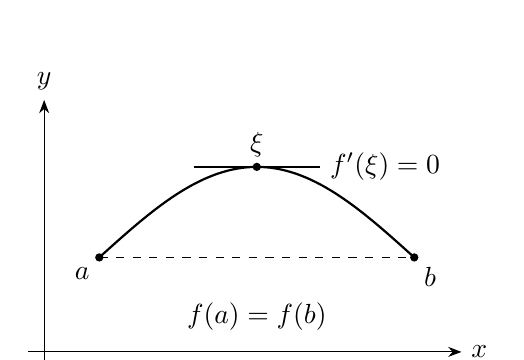
\begin{tikzpicture}[scale=1.0,>=Stealth]
  \draw[->] (-0.2,0)--(5.3,0) node[right] {$x$};
  \draw[->] (0,-0.2)--(0,3.2) node[above] {$y$};
  \draw[domain=0.7:4.7,smooth,variable=\x,thick]
    plot ({\x},{1.2+1.15*sin(45*(\x-0.7))});
  \coordinate (A) at (0.7,1.2);
  \coordinate (B) at (4.7,1.2);
  \coordinate (C) at (2.7,2.35);
  \fill (A) circle (1.5pt) node[below left] {$a$};
  \fill (B) circle (1.5pt) node[below right] {$b$};
  \fill (C) circle (1.5pt) node[above] {$\xi$};
  \draw[dashed] (A)--(B);
  \draw[thick] (1.9,2.35)--(3.5,2.35) node[right] {$f'(\xi)=0$};
  \node at (2.7,0.45) {$f(a)=f(b)$};
\end{tikzpicture}
\end{center}

\begin{theorem}[Lagrange 中值定理]
若 $f$ 在 $[a,b]$ 上连续，在 $(a,b)$ 内可导，则存在 $\xi\in(a,b)$，使得
\[
f'(\xi)=\frac{f(b)-f(a)}{b-a}.
\]
\end{theorem}
\begin{proofdetail}
构造辅助函数
\[
F(x)=f(x)-\frac{f(b)-f(a)}{b-a}(x-a).
\]
$F$ 在 $[a,b]$ 上连续，在 $(a,b)$ 内可导，且
\[
F(a)=f(a),\qquad F(b)=f(b)-[f(b)-f(a)]=f(a).
\]
由 Rolle 定理，存在 $\xi\in(a,b)$ 使 $F'(\xi)=0$. 而
\[
F'(x)=f'(x)-\frac{f(b)-f(a)}{b-a},
\]
故结论成立.
\end{proofdetail}

Lagrange 中值定理的几何意义是：连续光滑曲线上至少有一点的切线平行于连接两端点的弦. 公式
\[
f(b)-f(a)=f'(\xi)(b-a)
\]
说明“总改变量”等于某个中间点的瞬时变化率乘以区间长度.

\begin{center}
\begin{tikzpicture}[scale=1.0,>=Stealth]
  \draw[->] (-0.2,0)--(5.4,0) node[right] {$x$};
  \draw[->] (0,-0.2)--(0,4.0) node[above] {$y$};
  % y=0.18(x-2.2)^2+1, with a=0.8, b=4.6.
  % The secant slope equals f'(2.7)=0.18, so the tangent at xi=2.7 is parallel to the secant.
  \draw[domain=0.55:4.85,smooth,variable=\x,thick]
    plot ({\x},{0.18*(\x-2.2)*(\x-2.2)+1});
  \coordinate (A) at (0.8,1.353);
  \coordinate (B) at (4.6,2.037);
  \coordinate (C) at (2.7,1.045);
  \fill (A) circle (1.5pt) node[below left] {$(a,f(a))$};
  \fill (B) circle (1.5pt) node[above right] {$(b,f(b))$};
  \fill (C) circle (1.5pt) node[below] {$(\xi,f(\xi))$};
  \draw[thick,dashed] (A)--(B) node[midway,above,sloped] {弦};
  \draw[thick] ($(C)+(-1.2,-0.216)$)--($(C)+(1.2,0.216)$) node[right] {切线};
  \draw[dashed] (0.8,0)--(0.8,1.353);
  \draw[dashed] (2.7,0)--(2.7,1.045);
  \draw[dashed] (4.6,0)--(4.6,2.037);
  \node[below] at (0.8,0) {$a$};
  \node[below] at (2.7,0) {$\xi$};
  \node[below] at (4.6,0) {$b$};
\end{tikzpicture}
\end{center}

\begin{example}[验证中值定理]
对 $f(x)=x^2$ 在 $[1,3]$ 上求满足 Lagrange 中值定理的 $\xi$.
\end{example}
\begin{solution}
\[
\frac{f(3)-f(1)}{3-1}=\frac{9-1}{2}=4.
\]
因 $f'(x)=2x$，令 $2\xi=4$ 得 $\xi=2\in(1,3)$.
\end{solution}

\begin{example}[Rolle 定理的条件核查]
判断函数
\[
f(x)=|x|
\]
在区间 $[-1,1]$ 上能否应用 Rolle 定理.
\end{example}
\begin{solution}
首先，
\[
f(-1)=1,\qquad f(1)=1,
\]
两端函数值相等，且 $f$ 在 $[-1,1]$ 上连续. 但是 $f$ 在 $x=0$ 处不可导，因为
\[
\lim_{h\to0+}\frac{|h|-0}{h}=1,\qquad
\lim_{h\to0-}\frac{|h|-0}{h}=-1,
\]
左右导数不相等. 因此 $f$ 不满足“在 $(-1,1)$ 内可导”的条件，不能应用 Rolle 定理.
\end{solution}
\begin{warning}
Rolle 定理的结论不是只由 $f(a)=f(b)$ 推出. 连续性和开区间可导性缺一不可，本题图像有尖点，正好破坏了可导性.
\end{warning}

\begin{example}[Rolle 定理证明方程根的个数]
证明方程
\[
x^3-3x+1=0
\]
在区间 $(-2,2)$ 内有三个不同实根.
\end{example}
\begin{solution}
设
\[
f(x)=x^3-3x+1.
\]
计算得
\[
f(-2)=-1,\quad f(-1)=3,\quad f(0)=1,\quad f(1)=-1,\quad f(2)=3.
\]
由介值定理，区间 $(-2,-1)$、$(0,1)$、$(1,2)$ 内各至少有一个零点，所以 $(-2,2)$ 内至少有三个不同实根.

下面证明不可能有四个或更多不同实根. 若存在四个不同实根
\[
r_1<r_2<r_3<r_4,
\]
则在每个区间 $[r_i,r_{i+1}]$ 上，函数连续、开区间内可导，且两端函数值都为 $0$. 由 Rolle 定理，$f'$ 在 $(r_1,r_2)$、$(r_2,r_3)$、$(r_3,r_4)$ 内各至少有一个零点，因此 $f'$ 至少有三个不同零点. 但
\[
f'(x)=3x^2-3=3(x-1)(x+1)
\]
只有两个零点 $-1,1$，矛盾. 故方程在 $(-2,2)$ 内恰有三个不同实根.
\end{solution}

\begin{example}[构造辅助函数]
设 $f$ 在 $[0,1]$ 上连续，在 $(0,1)$ 内可导，且 $f(1)=0$. 证明存在 $\xi\in(0,1)$，使得
\[
f'(\xi)=-\frac{f(\xi)}{\xi}.
\]
\end{example}
\begin{solution}
令
\[
F(x)=xf(x).
\]
则 $F$ 在 $[0,1]$ 上连续，在 $(0,1)$ 内可导，并且
\[
F(0)=0,\qquad F(1)=f(1)=0.
\]
由 Rolle 定理，存在 $\xi\in(0,1)$，使得 $F'(\xi)=0$. 而
\[
F'(x)=f(x)+xf'(x),
\]
所以
\[
f(\xi)+\xi f'(\xi)=0.
\]
由于 $\xi\in(0,1)$，可除以 $\xi$，得到
\[
f'(\xi)=-\frac{f(\xi)}{\xi}.
\]
\end{solution}

\begin{example}[构造辅助函数]
设 $f$ 在 $[a,b]$ 上连续，在 $(a,b)$ 内可导，且 $f(a)=f(b)=0$. 证明存在 $\xi\in(a,b)$，使得
\[
f'(\xi)+f(\xi)=0.
\]
\end{example}
\begin{solution}
观察到表达式 $f'(x)+f(x)$ 是 $\ee^x f(x)$ 的导数中除去正因子后的部分. 令
\[
F(x)=\ee^x f(x).
\]
则 $F$ 在 $[a,b]$ 上连续，在 $(a,b)$ 内可导，并且
\[
F(a)=\ee^a f(a)=0,\qquad F(b)=\ee^b f(b)=0.
\]
由 Rolle 定理，存在 $\xi\in(a,b)$，使得 $F'(\xi)=0$. 而
\[
F'(x)=\ee^x f(x)+\ee^x f'(x)=\ee^x[f'(x)+f(x)].
\]
由于 $\ee^\xi>0$，所以
\[
f'(\xi)+f(\xi)=0.
\]
\end{solution}

\begin{example}[由导数界估计函数增量]
设 $f$ 在 $[a,b]$ 上连续，在 $(a,b)$ 内可导，且存在常数 $M>0$，使得
\[
|f'(x)|\leq M,\qquad x\in(a,b).
\]
证明对任意 $x_1,x_2\in[a,b]$，有
\[
|f(x_2)-f(x_1)|\leq M|x_2-x_1|.
\]
\end{example}
\begin{solution}
若 $x_1=x_2$，结论成立. 设 $x_1<x_2$. 由 Lagrange 中值定理，存在 $\xi\in(x_1,x_2)$，使得
\[
f(x_2)-f(x_1)=f'(\xi)(x_2-x_1).
\]
取绝对值得
\[
|f(x_2)-f(x_1)|=|f'(\xi)|\,|x_2-x_1|\leq M|x_2-x_1|.
\]
当 $x_1>x_2$ 时交换两点即可.
\end{solution}

\subsection{Cauchy 中值定理与若干推论}

\begin{theorem}[Cauchy 中值定理]
若 $f,g$ 在 $[a,b]$ 上连续，在 $(a,b)$ 内可导，且 $g'(x)\neq0$ 对所有 $x\in(a,b)$ 成立，则存在 $\xi\in(a,b)$，使得
\[
\frac{f'(\xi)}{g'(\xi)}=\frac{f(b)-f(a)}{g(b)-g(a)}.
\]
\end{theorem}
\begin{proofdetail}
先说明 $g(b)\neq g(a)$. 若 $g(b)=g(a)$，由 Rolle 定理存在 $\eta\in(a,b)$ 使 $g'(\eta)=0$，与条件矛盾.

构造
\[
F(x)=f(x)-f(a)-\frac{f(b)-f(a)}{g(b)-g(a)}[g(x)-g(a)].
\]
则 $F$ 在 $[a,b]$ 连续，在 $(a,b)$ 可导，且 $F(a)=F(b)=0$. 由 Rolle 定理，存在 $\xi\in(a,b)$ 使 $F'(\xi)=0$. 即
\[
f'(\xi)-\frac{f(b)-f(a)}{g(b)-g(a)}g'(\xi)=0.
\]
因 $g'(\xi)\neq0$，除以 $g'(\xi)$ 得结论.
\end{proofdetail}

\begin{proposition}[导数恒为零的函数为常数]
若 $f$ 在区间 $I$ 上可导，且 $f'(x)=0$ 对所有 $x\in I$ 成立，则 $f$ 在 $I$ 上为常数.
\end{proposition}
\begin{proofdetail}
任取 $x_1,x_2\in I$，不妨 $x_1<x_2$. $f$ 在 $[x_1,x_2]$ 连续、在 $(x_1,x_2)$ 可导. 由 Lagrange 中值定理，存在 $\xi\in(x_1,x_2)$ 使
\[
f(x_2)-f(x_1)=f'(\xi)(x_2-x_1)=0.
\]
故任意两点函数值相等，$f$ 为常数.
\end{proofdetail}

\begin{proposition}[导数相等的函数相差常数]
若 $f,g$ 在区间 $I$ 上可导，且
\[
f'(x)=g'(x),\qquad x\in I,
\]
则存在常数 $C$，使得
\[
f(x)=g(x)+C,\qquad x\in I.
\]
\end{proposition}
\begin{proofdetail}
令 $h(x)=f(x)-g(x)$. 则 $h$ 在 $I$ 上可导，且
\[
h'(x)=f'(x)-g'(x)=0.
\]
由“导数恒为零的函数为常数”，$h(x)=C$. 即
\[
f(x)-g(x)=C.
\]
\end{proofdetail}

\begin{example}[Cauchy 中值定理验证]
设
\[
f(x)=\ln x,\qquad g(x)=x,\qquad x\in[1,\ee].
\]
求 Cauchy 中值定理中的 $\xi$.
\end{example}
\begin{solution}
$f,g$ 在 $[1,\ee]$ 上连续，在 $(1,\ee)$ 内可导，且 $g'(x)=1\neq0$. Cauchy 中值定理给出存在 $\xi\in(1,\ee)$，使
\[
\frac{f'(\xi)}{g'(\xi)}
=\frac{f(\ee)-f(1)}{g(\ee)-g(1)}.
\]
即
\[
\frac{1/\xi}{1}=\frac{1-0}{\ee-1}=\frac1{\ee-1}.
\]
因此
\[
\xi=\ee-1.
\]
由于 $1<\ee-1<\ee$，该点确在区间内部.
\end{solution}

\begin{example}[用 Cauchy 中值定理证明不等式]
证明当 $0<a<b$ 时，
\[
\frac{b-a}{b}<\ln b-\ln a<\frac{b-a}{a}.
\]
\end{example}
\begin{solution}
对 $f(x)=\ln x$ 和 $g(x)=x$ 在 $[a,b]$ 上应用 Cauchy 中值定理，存在 $\xi\in(a,b)$，使得
\[
\frac{\ln b-\ln a}{b-a}=\frac{f'(\xi)}{g'(\xi)}=\frac1{\xi}.
\]
因为 $a<\xi<b$，所以
\[
\frac1b<\frac1\xi<\frac1a.
\]
又 $b-a>0$，两边同乘以 $b-a$ 得
\[
\frac{b-a}{b}<\ln b-\ln a<\frac{b-a}{a}.
\]
\end{solution}

\begin{example}[不等式]
证明当 $x>0$ 时，$\ln(1+x)<x$.
\end{example}
\begin{solution}
令 $f(t)=\ln(1+t)$，在 $[0,x]$ 上应用 Lagrange 中值定理，存在 $\xi\in(0,x)$ 使
\[
\ln(1+x)-\ln1=f'(\xi)x=\frac{x}{1+\xi}.
\]
因 $\xi>0$，有 $1+\xi>1$，故 $\ln(1+x)=x/(1+\xi)<x$.
\end{solution}

\begin{example}[不等式]
证明当 $x>0$ 时，
\[
\ln(1+x)>\frac{x}{1+x}.
\]
\end{example}
\begin{solution}
令
\[
F(x)=\ln(1+x)-\frac{x}{1+x},\qquad x\geq0.
\]
有 $F(0)=0$，且当 $x>0$ 时
\[
F'(x)=\frac1{1+x}-\frac1{(1+x)^2}
=\frac{x}{(1+x)^2}>0.
\]
由单调性判别法，$F$ 在 $[0,\infty)$ 上单调增加. 因此对 $x>0$，
\[
F(x)>F(0)=0,
\]
即
\[
\ln(1+x)>\frac{x}{1+x}.
\]
\end{solution}

\begin{example}[三角函数不等式]
证明当 $x>0$ 时，
\[
\sin x<x.
\]
\end{example}
\begin{solution}
当 $x\geq\pi$ 时，$\sin x\leq1<x$，结论成立. 下面只需考虑 $0<x<\pi$.

令 $f(t)=\sin t$，在 $[0,x]$ 上应用 Lagrange 中值定理，存在 $\xi\in(0,x)$，使得
\[
\sin x-\sin0=f'(\xi)x=\cos\xi\,x.
\]
由于 $0<\xi<\pi$，有 $\cos\xi<1$，故
\[
\sin x=x\cos\xi<x.
\]
\end{solution}

\begin{example}[指数函数不等式]
证明对一切实数 $x$，
\[
\ee^x\geq1+x,
\]
且等号当且仅当 $x=0$.
\end{example}
\begin{solution}
令
\[
F(x)=\ee^x-1-x.
\]
则
\[
F'(x)=\ee^x-1.
\]
当 $x<0$ 时，$F'(x)<0$；当 $x>0$ 时，$F'(x)>0$. 因而 $F$ 在 $(-\infty,0)$ 上单调减少，在 $(0,\infty)$ 上单调增加，所以 $x=0$ 是全局最小点. 又
\[
F(0)=0.
\]
于是 $F(x)\geq0$，即
\[
\ee^x\geq1+x.
\]
当 $x\neq0$ 时，$F(x)>F(0)=0$，故等号仅当 $x=0$ 成立.
\end{solution}

\subsection{洛必达法则}

\begin{theorem}[洛必达法则：$0/0$ 型]
设 $f,g$ 在 $a$ 的某去心右邻域内可导，且 $g'(x)\neq0$. 若
\[
\lim_{x\to a+}f(x)=\lim_{x\to a+}g(x)=0,\qquad
\lim_{x\to a+}\frac{f'(x)}{g'(x)}=L
\]
其中 $L$ 可为有限数或无穷大，则
\[
\lim_{x\to a+}\frac{f(x)}{g(x)}=L.
\]
左极限、双侧极限与 $x\to\infty$ 的相应形式类似成立.
\end{theorem}
\begin{proofdetail}
先证 $L$ 为有限数的情形. 任取 $\varepsilon>0$，由 $\frac{f'}{g'}\to L$，存在 $\delta>0$，当 $a<x<a+\delta$ 时，
\[
L-\varepsilon<\frac{f'(x)}{g'(x)}<L+\varepsilon.
\]
取 $x\in(a,a+\delta)$，再取 $t\in(a,x)$. 在 $[t,x]$ 上对 $f,g$ 应用 Cauchy 中值定理，存在 $\xi\in(t,x)$ 使
\[
\frac{f(x)-f(t)}{g(x)-g(t)}=\frac{f'(\xi)}{g'(\xi)}.
\]
因此
\[
\left|\frac{f(x)-f(t)}{g(x)-g(t)}-L\right|<\varepsilon.
\]
固定 $x$ 后令 $t\to a+$，由 $f(t)\to0,g(t)\to0$ 得
\[
\left|\frac{f(x)}{g(x)}-L\right|\leq\varepsilon
\]
其中 $x\in(a,a+\delta)$ 且 $g(x)\neq0$. 因 $\varepsilon$ 任意，得 $\frac{f(x)}{g(x)}\to L$.

若 $L=+\infty$，对任意 $M>0$，存在 $\delta>0$ 使 $a<x<a+\delta$ 时 $\frac{f'(x)}{g'(x)}>M$. 重复上面的 Cauchy 中值定理步骤，令 $t\to a+$ 得 $\frac{f(x)}{g(x)}>M$，故极限为 $+\infty$. $L=-\infty$ 同理.
\end{proofdetail}

\begin{theorem}[洛必达法则：$\infty/\infty$ 型]
设 $f,g$ 在 $a$ 的某去心右邻域内可导，且 $g'(x)\neq0$. 若
\[
\lim_{x\to a+}|f(x)|=+\infty,\qquad
\lim_{x\to a+}|g(x)|=+\infty,
\]
并且
\[
\lim_{x\to a+}\frac{f'(x)}{g'(x)}=L,
\]
其中 $L$ 可为有限数或无穷大，则
\[
\lim_{x\to a+}\frac{f(x)}{g(x)}=L.
\]
左极限、双侧极限与 $x\to\infty$ 的相应形式类似成立.
\end{theorem}
\begin{proofdetail}
证明有限 $L$ 的情形. 任取 $\varepsilon>0$，由 $\frac{f'}{g'}\to L$，存在去心右邻域，使得其中任意点 $u$ 都满足
\[
\left|\frac{f'(u)}{g'(u)}-L\right|<\varepsilon.
\]
固定该邻域内一点 $x_0$. 对 $x$ 与 $x_0$ 之间的闭区间应用 Cauchy 中值定理，存在 $\xi$ 介于 $x$ 与 $x_0$ 之间，使
\[
\frac{f(x)-f(x_0)}{g(x)-g(x_0)}=\frac{f'(\xi)}{g'(\xi)}.
\]
当 $x\to a+$ 时，$\xi\to a+$，所以
\[
\frac{f(x)-f(x_0)}{g(x)-g(x_0)}\to L.
\]
又因为 $|f(x)|,|g(x)|\to\infty$，有
\[
\frac{f(x)}{g(x)}
=\frac{f(x)-f(x_0)}{g(x)-g(x_0)}
\cdot
\frac{1-\frac{f(x_0)}{f(x)}}{1-\frac{g(x_0)}{g(x)}}.
\]
第二个因子趋于 $1$，故 $\frac{f(x)}{g(x)}\to L$. $L$ 为无穷大的情形可仿照 $0/0$ 型证明，用任意大数估计完成.
\end{proofdetail}

\begin{example}[$0/0$ 型]
求 $\displaystyle\lim_{x\to0}\frac{\sin x}{x}$.
\end{example}
\begin{solution}
这是 $0/0$ 型. 用洛必达法则：
\[
\lim_{x\to0}\frac{\sin x}{x}=\lim_{x\to0}\frac{\cos x}{1}=1.
\]
\end{solution}

\begin{example}[多次使用]
求 $\displaystyle\lim_{x\to0}\frac{\ee^x-1-x}{x^2}$.
\end{example}
\begin{solution}
第一次洛必达：
\[
\lim_{x\to0}\frac{\ee^x-1-x}{x^2}
=\lim_{x\to0}\frac{\ee^x-1}{2x}.
\]
仍为 $0/0$ 型，第二次洛必达：
\[
=\lim_{x\to0}\frac{\ee^x}{2}=\frac12.
\]
\end{solution}
\begin{warning}
使用洛必达前必须确认是 $0/0$ 或 $\infty/\infty$ 型，并确认分母导数不为零的条件在去心邻域内成立.
\end{warning}

\begin{example}[$\infty/\infty$ 型]
求
\[
\lim_{x\to\infty}\frac{\ln x}{x^\alpha},\qquad \alpha>0.
\]
\end{example}
\begin{solution}
当 $x\to\infty$ 时，分子、分母都趋于 $+\infty$，属于 $\infty/\infty$ 型. 用洛必达法则：
\[
\lim_{x\to\infty}\frac{\ln x}{x^\alpha}
=\lim_{x\to\infty}\frac{1/x}{\alpha x^{\alpha-1}}
=\lim_{x\to\infty}\frac{1}{\alpha x^\alpha}=0.
\]
这说明任意正幂函数 $x^\alpha$ 的增长都快于 $\ln x$.
\end{solution}

\begin{example}[三角函数高阶小量]
求
\[
\lim_{x\to0}\frac{\tan x-x}{x^3}.
\]
\end{example}
\begin{solution}
这是 $0/0$ 型. 第一次洛必达：
\[
\lim_{x\to0}\frac{\tan x-x}{x^3}
=\lim_{x\to0}\frac{\sec^2x-1}{3x^2}
=\lim_{x\to0}\frac{\tan^2x}{3x^2}.
\]
因为 $\lim_{x\to0}\frac{\tan x}{x}=1$，所以
\[
\lim_{x\to0}\frac{\tan^2x}{3x^2}
=\frac13.
\]
\end{solution}

\begin{example}[不能机械使用洛必达法则]
讨论 $\displaystyle\lim_{x\to\infty}\frac{x+\sin x}{x+\cos x}$.
\end{example}
\begin{solution}
这是 $\infty/\infty$ 型，但直接看导数之比会得到
\[
\frac{(x+\sin x)'}{(x+\cos x)'}=\frac{1+\cos x}{1-\sin x},
\]
该式当 $x\to\infty$ 时无极限，因此不能由洛必达法则推出原极限不存在. 原式应先整理：
\[
\frac{x+\sin x}{x+\cos x}
=\frac{1+\frac{\sin x}{x}}{1+\frac{\cos x}{x}}.
\]
由于 $\sin x/x\to0,\ \cos x/x\to0$，原极限为 $1$.
\end{solution}
\begin{warning}
洛必达法则给出的是充分条件：若导数之比的极限存在，原比值极限等于它. 导数之比极限不存在时，原极限仍可能存在.
\end{warning}

\begin{example}[转化未定式]
求 $\displaystyle\lim_{x\to0+}x\ln x$.
\end{example}
\begin{solution}
原式为 $0\cdot(-\infty)$ 型，改写为
\[
x\ln x=\frac{\ln x}{1/x}.
\]
当 $x\to0+$ 时为 $-\infty/\infty$ 型. 用洛必达法则：
\[
\lim_{x\to0+}\frac{\ln x}{1/x}
=\lim_{x\to0+}\frac{1/x}{-1/x^2}
=\lim_{x\to0+}(-x)=0.
\]
\end{solution}

\begin{example}[指数型未定式]
求
\[
\lim_{x\to0+}x^x.
\]
\end{example}
\begin{solution}
原式为 $0^0$ 型. 设
\[
y=x^x.
\]
取对数得
\[
\ln y=x\ln x.
\]
由上一例，
\[
\lim_{x\to0+}x\ln x=0.
\]
因此
\[
\lim_{x\to0+}\ln y=0.
\]
由于指数函数连续，
\[
\lim_{x\to0+}x^x=\ee^0=1.
\]
\end{solution}

\begin{example}[差型未定式]
求
\[
\lim_{x\to0+}\left(\frac1x-\frac1{\ee^x-1}\right).
\]
\end{example}
\begin{solution}
原式为 $\infty-\infty$ 型，先通分：
\[
\frac1x-\frac1{\ee^x-1}
=\frac{\ee^x-1-x}{x(\ee^x-1)}.
\]
当 $x\to0+$ 时为 $0/0$ 型. 用洛必达法则：
\[
\lim_{x\to0+}\frac{\ee^x-1-x}{x(\ee^x-1)}
=\lim_{x\to0+}\frac{\ee^x-1}{\ee^x-1+x\ee^x}.
\]
仍为 $0/0$ 型，再用一次洛必达：
\[
=\lim_{x\to0+}\frac{\ee^x}{2\ee^x+x\ee^x}
=\frac12.
\]
\end{solution}

\begin{example}[参数型极限]
设 $a>0$. 求
\[
\lim_{x\to0}\frac{a^x-1}{x}.
\]
\end{example}
\begin{solution}
当 $x\to0$ 时为 $0/0$ 型. 由洛必达法则，
\[
\lim_{x\to0}\frac{a^x-1}{x}
=\lim_{x\to0}\frac{a^x\ln a}{1}
=\ln a.
\]
特别地，当 $a=\ee$ 时，得到
\[
\lim_{x\to0}\frac{\ee^x-1}{x}=1.
\]
\end{solution}

\subsection{课后习题}
\begin{enumerate}[label=\textbf{练习\arabic*.},leftmargin=2.2em]
\item 判断下列函数在给定区间上能否应用 Rolle 定理；若能，求出满足结论的点：
\[
f(x)=x^2-1,\ [-1,1];\qquad
g(x)=|x|,\ [-1,1].
\]
\item 对函数 $f(x)=x^3$ 在区间 $[-1,2]$ 上求满足 Lagrange 中值定理的 $\xi$.
\item 设 $f$ 在 $[0,1]$ 上连续，在 $(0,1)$ 内可导，且 $f(0)=f(1)$. 证明存在 $\xi\in(0,1)$，使得
\[
f'(\xi)=0.
\]
\item 设 $f$ 在 $[a,b]$ 上连续，在 $(a,b)$ 内可导，且 $f(a)=f(b)=0$. 证明存在 $\xi\in(a,b)$，使得
\[
f'(\xi)+f(\xi)=0.
\]
\item 证明当 $x>0$ 时，
\[
\frac{x}{1+x}<\ln(1+x)<x.
\]
\item 证明对一切实数 $x$，有
\[
\ee^x\geq1+x.
\]
\item 证明当 $0<a<b$ 时，
\[
\frac{b-a}{b}<\ln b-\ln a<\frac{b-a}{a}.
\]
\item 求极限：
\[
\lim_{x\to0}\frac{\tan x-x}{x^3},\qquad
\lim_{x\to0}\frac{\ee^x-1-x}{x^2}.
\]
\item 求极限：
\[
\lim_{x\to\infty}\frac{\ln x}{\sqrt{x}},\qquad
\lim_{x\to0+}x\ln x.
\]
\item 求极限：
\[
\lim_{x\to0+}x^x,\qquad
\lim_{x\to0+}\left(\frac1x-\frac1{\ee^x-1}\right).
\]
\item 设 $a>0$，求
\[
\lim_{x\to0}\frac{a^x-1}{x}.
\]
\item 讨论
\[
\lim_{x\to\infty}\frac{x+\sin x}{x+\cos x},
\]
并说明为什么不能因导数之比无极限就断定原极限不存在.
\end{enumerate}

\subsection{参考解答}
\begin{enumerate}[label=\textbf{练习\arabic*.},leftmargin=2.2em]
\item $f(x)=x^2-1$ 在 $[-1,1]$ 上连续、在 $(-1,1)$ 内可导，且 $f(-1)=f(1)=0$，可用 Rolle 定理. 由
\[
f'(x)=2x
\]
得 $\xi=0$. 函数 $g(x)=|x|$ 虽在 $[-1,1]$ 上连续且 $g(-1)=g(1)$，但在 $0$ 处不可导，不能应用 Rolle 定理.
\item
\[
\frac{f(2)-f(-1)}{2-(-1)}=\frac{8-(-1)}{3}=3.
\]
而 $f'(x)=3x^2$，令 $3\xi^2=3$，得 $\xi=\pm1$. 由于 $\xi\in(-1,2)$，故只有 $\xi=1$ 满足.
\item 这正是 Rolle 定理. 由于 $f$ 在 $[0,1]$ 上连续、在 $(0,1)$ 内可导，且 $f(0)=f(1)$，存在 $\xi\in(0,1)$ 使 $f'(\xi)=0$.
\item 令 $F(x)=\ee^x f(x)$. 则 $F(a)=F(b)=0$，由 Rolle 定理存在 $\xi$ 使
\[
F'(\xi)=\ee^\xi[f'(\xi)+f(\xi)]=0.
\]
由于 $\ee^\xi>0$，故 $f'(\xi)+f(\xi)=0$.
\item 左侧可令
\[
F(x)=\ln(1+x)-\frac{x}{1+x}.
\]
则 $F(0)=0$，且
\[
F'(x)=\frac{x}{(1+x)^2}>0\qquad(x>0),
\]
所以 $F(x)>0$. 右侧由 Lagrange 中值定理得
\[
\ln(1+x)=\frac{x}{1+\xi}<x,\qquad 0<\xi<x.
\]
\item 令 $F(x)=\ee^x-1-x$. 则 $F'(x)=\ee^x-1$. $F$ 在 $(-\infty,0)$ 上递减，在 $(0,\infty)$ 上递增，故 $F(0)=0$ 为全局最小值. 因此 $\ee^x\geq1+x$.
\item 对 $f(x)=\ln x$、$g(x)=x$ 在 $[a,b]$ 上应用 Cauchy 中值定理，存在 $\xi\in(a,b)$，使
\[
\frac{\ln b-\ln a}{b-a}=\frac1\xi.
\]
由 $a<\xi<b$，得
\[
\frac1b<\frac1\xi<\frac1a.
\]
同乘 $b-a>0$ 即得结论.
\item
\[
\lim_{x\to0}\frac{\tan x-x}{x^3}
=\lim_{x\to0}\frac{\sec^2x-1}{3x^2}
=\lim_{x\to0}\frac{\tan^2x}{3x^2}=\frac13.
\]
又
\[
\lim_{x\to0}\frac{\ee^x-1-x}{x^2}
=\lim_{x\to0}\frac{\ee^x-1}{2x}
=\lim_{x\to0}\frac{\ee^x}{2}=\frac12.
\]
\item
\[
\lim_{x\to\infty}\frac{\ln x}{\sqrt{x}}
=\lim_{x\to\infty}\frac{1/x}{1/(2\sqrt{x})}
=\lim_{x\to\infty}\frac{2}{\sqrt{x}}=0.
\]
另外
\[
\lim_{x\to0+}x\ln x
=\lim_{x\to0+}\frac{\ln x}{1/x}
=\lim_{x\to0+}\frac{1/x}{-1/x^2}
=\lim_{x\to0+}(-x)=0.
\]
\item
\[
x^x=\ee^{x\ln x},\qquad x\ln x\to0,
\]
所以 $\lim_{x\to0+}x^x=1$. 其次
\[
\frac1x-\frac1{\ee^x-1}
=\frac{\ee^x-1-x}{x(\ee^x-1)}.
\]
两次洛必达得
\[
\lim_{x\to0+}\frac{\ee^x-1-x}{x(\ee^x-1)}
=\lim_{x\to0+}\frac{\ee^x-1}{\ee^x-1+x\ee^x}
=\lim_{x\to0+}\frac{\ee^x}{2\ee^x+x\ee^x}
=\frac12.
\]
\item
\[
\lim_{x\to0}\frac{a^x-1}{x}
=\lim_{x\to0}a^x\ln a=\ln a.
\]
\item
\[
\frac{x+\sin x}{x+\cos x}
=\frac{1+\frac{\sin x}{x}}{1+\frac{\cos x}{x}}\to1.
\]
导数之比为
\[
\frac{1+\cos x}{1-\sin x},
\]
它没有极限. 洛必达法则只能说“若导数之比极限存在，则原极限等于它”，不能反过来由导数之比无极限推出原极限不存在.
\end{enumerate}

\section{导数的应用}
\renewEnvironmentCounter
\subsection{函数单调性判别法}

\begin{theorem}[单调性判别法]
设 $f$ 在区间 $I$ 上连续，在 $I$ 的内部可导. 若 $f'(x)\geq0$ 对内部所有点成立，则 $f$ 在 $I$ 上单调不减；若 $f'(x)>0$ 对内部所有点成立，则 $f$ 在 $I$ 上严格单调增加. 相应地，$f'(x)\leq0$ 推出单调不增，$f'(x)<0$ 推出严格单调减少.
\end{theorem}
\begin{proofdetail}
任取 $x_1<x_2$，由 Lagrange 中值定理，存在 $\xi\in(x_1,x_2)$，使
\[
f(x_2)-f(x_1)=f'(\xi)(x_2-x_1).
\]
若 $f'\geq0$，则右端 $\geq0$，故 $f(x_2)\geq f(x_1)$. 若 $f'>0$，则右端 $>0$，故严格增加. 其余情形同理.
\end{proofdetail}

\begin{example}[求单调区间]
求 $f(x)=x^3-3x$ 的单调区间.
\end{example}
\begin{solution}
\[
f'(x)=3x^2-3=3(x-1)(x+1).
\]
当 $x<-1$ 或 $x>1$ 时 $f'(x)>0$；当 $-1<x<1$ 时 $f'(x)<0$. 故 $f$ 在 $(-\infty,-1)$ 与 $(1,\infty)$ 上单调增加，在 $(-1,1)$ 上单调减少.
\end{solution}

\begin{example}[求单调区间]
求函数
\[
f(x)=2x^3-9x^2+12x-3
\]
的单调区间.
\end{example}
\begin{solution}
\[
f'(x)=6x^2-18x+12=6(x-1)(x-2).
\]
临界点为 $x=1,2$. 当 $x<1$ 时 $f'(x)>0$；当 $1<x<2$ 时 $f'(x)<0$；当 $x>2$ 时 $f'(x)>0$. 因此 $f$ 在 $(-\infty,1)$ 与 $(2,\infty)$ 上单调增加，在 $(1,2)$ 上单调减少.
\end{solution}

\subsection{函数的极值}

\begin{definition}[局部极值]
若存在 $\delta>0$，使得对所有满足 $|x-x_0|<\delta$ 的 $x$，都有 $f(x)\leq f(x_0)$，则称 $f(x_0)$ 为局部极大值. 若不等号反向，则称为局部极小值.
\end{definition}

\begin{theorem}[一阶导数变号判别法]
设 $f$ 在 $x_0$ 连续，在 $x_0$ 的去心邻域内可导. 若 $f'$ 在 $x_0$ 左侧为正、右侧为负，则 $f(x_0)$ 为局部极大值；若左侧为负、右侧为正，则为局部极小值；若左右不变号，则不是极值点.
\end{theorem}
\begin{proofdetail}
只证由正变负的情形. 存在 $\delta>0$，使 $f'(x)>0$ 对 $x\in(x_0-\delta,x_0)$ 成立，$f'(x)<0$ 对 $x\in(x_0,x_0+\delta)$ 成立. 由单调性判别法，$f$ 在左侧区间单调增加，在右侧区间单调减少. 因 $f$ 在 $x_0$ 连续，对任意 $x\in(x_0-\delta,x_0)$ 有 $f(x)<f(x_0)$，对任意 $x\in(x_0,x_0+\delta)$ 有 $f(x)<f(x_0)$. 因此 $f(x_0)$ 为局部极大值. 其余情形同理.
\end{proofdetail}

\begin{theorem}[二阶导数判别法]
设 $f'(x_0)=0$，且 $f''(x_0)$ 存在. 若 $f''(x_0)>0$，则 $f(x_0)$ 是局部极小值；若 $f''(x_0)<0$，则是局部极大值.
\end{theorem}
\begin{proofdetail}
由二阶导数定义，
\[
f''(x_0)=\lim_{x\to x_0}\frac{f'(x)-f'(x_0)}{x-x_0}
=\lim_{x\to x_0}\frac{f'(x)}{x-x_0}.
\]
若 $f''(x_0)>0$，则存在 $\delta>0$，当 $0<|x-x_0|<\delta$ 时
\[
\frac{f'(x)}{x-x_0}>0.
\]
于是 $x<x_0$ 时 $f'(x)<0$，$x>x_0$ 时 $f'(x)>0$，由一阶变号判别法得局部极小. $f''(x_0)<0$ 时同理得到导数由正变负，故为局部极大.
\end{proofdetail}

\begin{example}[极值]
求 $f(x)=x^4-4x^3$ 的极值.
\end{example}
\begin{solution}
\[
f'(x)=4x^3-12x^2=4x^2(x-3).
\]
临界点为 $x=0,3$. 因 $x^2\geq0$，$f'(x)$ 在 $0$ 两侧均为负，所以 $x=0$ 不是极值点. $f'$ 在 $3$ 左侧负、右侧正，故 $x=3$ 为局部极小点，
\[
f(3)=81-108=-27.
\]
\end{solution}
\begin{warning}
导数为零只是极值的必要条件，不是充分条件. $x=0$ 就是典型反例.
\end{warning}

\begin{example}[极值]
求函数
\[
f(x)=(x-1)^2(x+1)^3
\]
的极值.
\end{example}
\begin{solution}
求导得
\[
f'(x)=2(x-1)(x+1)^3+3(x-1)^2(x+1)^2
=(x-1)(x+1)^2(5x-1).
\]
临界点为 $x=-1,\frac15,1$. 由于 $(x+1)^2\geq0$，且除 $x=-1$ 外不改变符号，只需考察 $(x-1)(5x-1)$ 的符号，并注意 $x=-1$ 两侧符号是否改变.

当 $x<\frac15$ 且 $x\neq-1$ 时，$(x-1)<0,\ 5x-1<0$，故 $f'(x)>0$；当 $\frac15<x<1$ 时，$f'(x)<0$；当 $x>1$ 时，$f'(x)>0$. 因而 $x=-1$ 不是极值点，$x=\frac15$ 为局部极大点，$x=1$ 为局部极小点.

函数值为
\[
f\left(\frac15\right)=\left(-\frac45\right)^2\left(\frac65\right)^3=\frac{3456}{3125},\qquad
f(1)=0.
\]
故局部极大值为 $\frac{3456}{3125}$，局部极小值为 $0$.
\end{solution}

\subsection{函数的最值与应用优化}

\begin{proposition}[闭区间最值求法]
若 $f$ 在 $[a,b]$ 连续，则最大值和最小值只能在端点、不可导点或内部驻点 $f'(x)=0$ 处取得. 逐一比较这些点的函数值即可.
\end{proposition}
\begin{proofdetail}
最值存在性来自闭区间连续函数最值定理. 若最值在内部点 $x_0$ 取得且 $f$ 在 $x_0$ 可导，则由 Fermat 引理 $f'(x_0)=0$. 若内部点不可导，也必须列入候选. 端点处 Fermat 引理不适用，因此端点也必须比较.
\end{proofdetail}

\begin{example}[利润最大化]
某产品价格与销量满足 $p(q)=100-q$，成本 $C(q)=20q+100$，其中 $0\leq q\leq100$. 求最大利润.
\end{example}
\begin{solution}
收入 $R(q)=qp(q)=100q-q^2$，利润
\[
\Pi(q)=R(q)-C(q)=80q-q^2-100.
\]
\[
\Pi'(q)=80-2q.
\]
令 $\Pi'(q)=0$ 得 $q=40$. 比较
\[
\Pi(0)=-100,\quad \Pi(40)=1600-100=1500,\quad \Pi(100)=8000-10000-100=-2100.
\]
最大利润为 $1500$，在 $q=40$ 时取得.
\end{solution}

\begin{example}[证明方程根的个数]
证明方程 $x^3-3x+1=0$ 在区间 $(-2,2)$ 内有三个不同实根.
\end{example}
\begin{solution}
设 $f(x)=x^3-3x+1$. 有
\[
f(-2)=-1,\quad f(-1)=3,\quad f(0)=1,\quad f(1)=-1,\quad f(2)=3.
\]
由介值定理，$(-2,-1)$、$(0,1)$、$(1,2)$ 内各至少有一个根.

再证至多三个根. 若有四个不同实根 $r_1<r_2<r_3<r_4$，由 Rolle 定理，$f'$ 在三个相邻根之间至少有三个不同零点. 但
\[
f'(x)=3x^2-3
\]
只有两个零点 $\pm1$，矛盾. 故恰有三个不同实根.
\end{solution}

\subsection{课后习题（一）：单调性、极值与最值}
\begin{enumerate}[label=\textbf{练习\arabic*.},leftmargin=2.2em]
\item 求函数 $f(x)=x+\frac1x$ 在 $(0,\infty)$ 上的最小值.
\item 证明 $\ee^x\geq1+x$，并说明等号何时成立.
\item 求 $y=x^3-6x^2+9x+1$ 的单调区间和极值.
\end{enumerate}

\subsection{参考解答（一）}
\begin{enumerate}[label=\textbf{练习\arabic*.},leftmargin=2.2em]
\item
\[
f'(x)=1-\frac1{x^2}.
\]
当 $0<x<1$ 时 $f'<0$，当 $x>1$ 时 $f'>0$，故 $x=1$ 处取最小值 $2$.
\item 令 $F(x)=\ee^x-1-x$. 则 $F'(x)=\ee^x-1$，$F$ 在 $(-\infty,0)$ 上递减，在 $(0,\infty)$ 上递增，故 $F(0)=0$ 为最小值. 等号仅当 $x=0$ 成立.
\item
\[
y'=3x^2-12x+9=3(x-1)(x-3).
\]
函数在 $(-\infty,1)$、$(3,\infty)$ 上增加，在 $(1,3)$ 上减少. $x=1$ 为局部极大点，$y(1)=5$；$x=3$ 为局部极小点，$y(3)=1$.
\end{enumerate}

\subsection{曲线的凸性与拐点}

\begin{definition}[曲线的上凸与下凸]
设曲线 $y=f(x)$ 在区间 $(a,b)$ 内每一点都有切线. 若曲线上任意一点处的切线都在曲线的上方，则称曲线在 $(a,b)$ 内为\textbf{上凸}；若曲线上任意一点处的切线都在曲线的下方，则称曲线在 $(a,b)$ 内为\textbf{下凸}.

教材之间关于“凸”“凹”的命名不完全一致. 本讲义在本节采用曲线的上凸、下凸说法，避免与现代凸分析中“凸函数”定义混淆.
\end{definition}

\begin{center}
\begin{tikzpicture}[scale=0.95,>=Stealth]
  \begin{scope}
    \draw[->] (-2.1,0)--(2.2,0) node[right] {$x$};
    \draw[->] (0,-0.3)--(0,2.7) node[above] {$y$};
    \draw[domain=-1.65:1.65,smooth,variable=\x,thick]
      plot ({\x},{0.42*\x*\x+0.45});
    \coordinate (P) at (0.75,0.686);
    \draw[thick] ($(P)+(-1.35,-0.851)$)--($(P)+(1.35,0.851)$);
    \fill (P) circle (1.5pt);
    \node at (0,-0.65) {下凸：切线在曲线下方};
  \end{scope}
  \begin{scope}[xshift=7cm]
    \draw[->] (-2.1,0)--(2.2,0) node[right] {$x$};
    \draw[->] (0,-0.3)--(0,2.7) node[above] {$y$};
    \draw[domain=-1.65:1.65,smooth,variable=\x,thick]
      plot ({\x},{2.25-0.42*\x*\x});
    \coordinate (Q) at (0.75,2.014);
    \draw[thick] ($(Q)+(-1.35,0.851)$)--($(Q)+(1.35,-0.851)$);
    \fill (Q) circle (1.5pt);
    \node at (0,-0.65) {上凸：切线在曲线上方};
  \end{scope}
\end{tikzpicture}
\end{center}

\begin{theorem}[二阶导数判别凸性]
若 $f$ 在 $(a,b)$ 内二阶可导，则：
\[
f''(x)>0\quad (x\in(a,b))\quad\Longrightarrow\quad y=f(x)\text{ 在 }(a,b)\text{ 内下凸};
\]
\[
f''(x)<0\quad (x\in(a,b))\quad\Longrightarrow\quad y=f(x)\text{ 在 }(a,b)\text{ 内上凸}.
\]
\end{theorem}
\begin{proofdetail}
只证 $f''>0$ 的情形. 任取 $x_0\in(a,b)$，点 $(x_0,f(x_0))$ 处切线为
\[
T(x)=f(x_0)+f'(x_0)(x-x_0).
\]
令
\[
F(x)=f(x)-T(x).
\]
则 $F(x_0)=0,\ F'(x_0)=0$，且
\[
F''(x)=f''(x)>0.
\]
由单调性判别法，$F'$ 在 $(a,b)$ 内严格增加. 因 $F'(x_0)=0$，当 $x<x_0$ 时 $F'(x)<0$，当 $x>x_0$ 时 $F'(x)>0$. 因此 $F$ 在 $x_0$ 左侧随 $x$ 增大而减少，在 $x_0$ 右侧随 $x$ 增大而增加. 对任意 $x\neq x_0$，都有 $F(x)>F(x_0)=0$，即
\[
f(x)>f(x_0)+f'(x_0)(x-x_0).
\]
这说明切线在曲线下方，故曲线下凸. 若 $f''<0$，则对 $-f$ 应用已证结论，得到原曲线切线在曲线上方，故上凸.
\end{proofdetail}

\begin{definition}[拐点]
若曲线 $y=f(x)$ 在点 $x_0$ 的两侧凸凹性发生改变，则称 $(x_0,f(x_0))$ 为曲线的拐点.
\end{definition}

\begin{center}
\begin{tikzpicture}[scale=1.0,>=Stealth]
  \draw[->] (-2.6,0)--(2.7,0) node[right] {$x$};
  \draw[->] (0,0.2)--(0,3.4) node[above] {$y$};
  \draw[domain=-2.05:2.05,smooth,variable=\x,thick]
    plot ({\x},{1.75+0.18*\x*\x*\x});
  \coordinate (I) at (0,1.75);
  \fill (I) circle (1.5pt) node[above left] {拐点};
  \draw[dashed] (0,0)--(I);
  \node at (-1.55,2.55) {上凸};
  \node at (1.45,1.0) {下凸};
  \node[below] at (0,0) {$x_0$};
\end{tikzpicture}
\end{center}

\begin{example}[凸性与拐点]
讨论 $f(x)=x^3-3x$ 的凸性与拐点.
\end{example}
\begin{solution}
\[
f''(x)=6x.
\]
当 $x<0$ 时 $f''(x)<0$，曲线上凸；当 $x>0$ 时 $f''(x)>0$，曲线下凸. 上凸、下凸性在 $x=0$ 改变，故 $(0,0)$ 是拐点.
\end{solution}

\begin{example}[凸性与拐点]
求曲线
\[
y=2x^3+3x^2+12x+14
\]
的上凸区间、下凸区间和拐点.
\end{example}
\begin{solution}
\[
y'=6x^2+6x+12,\qquad y''=12x+6=6(2x+1).
\]
令 $y''=0$ 得 $x=-\frac12$. 当 $x<-\frac12$ 时 $y''<0$，曲线上凸；当 $x>-\frac12$ 时 $y''>0$，曲线下凸. 因此上凸区间为
\[
\left(-\infty,-\frac12\right),
\]
下凸区间为
\[
\left(-\frac12,\infty\right).
\]
又
\[
y\left(-\frac12\right)=2\left(-\frac18\right)+3\left(\frac14\right)+12\left(-\frac12\right)+14
=\frac{17}{2}.
\]
所以拐点为
\[
\left(-\frac12,\frac{17}{2}\right).
\]
\end{solution}

\subsection{曲线的渐近线与函数图像}

\begin{definition}[渐近线]
若 $\lim_{x\to x_0}f(x)=\infty$ 或 $-\infty$，则 $x=x_0$ 为垂直渐近线. 若 $\lim_{x\to\infty}f(x)=b$，则 $y=b$ 为水平渐近线. 若存在 $a,b$ 使
\[
\lim_{x\to\infty}[f(x)-(ax+b)]=0,
\]
则 $y=ax+b$ 为斜渐近线. $x\to-\infty$ 时同理.
\end{definition}

\begin{center}
\begin{tikzpicture}[scale=0.95,>=Stealth]
  \begin{scope}
    \draw[->] (-1.6,0)--(3.2,0) node[right] {$x$};
    \draw[->] (0,-1.1)--(0,3.0) node[above] {$y$};
    \draw[dashed] (1,-1.0)--(1,2.8) node[above] {$x=x_0$};
    \draw[dashed] (-1.5,1)--(3.0,1) node[right] {$y=b$};
    \draw[domain=-1.4:0.72,smooth,variable=\x,thick]
      plot ({\x},{1+0.55/(\x-1)});
    \draw[domain=1.28:3.0,smooth,variable=\x,thick]
      plot ({\x},{1+0.55/(\x-1)});
    \node at (0.75,-1.45) {垂直渐近线与水平渐近线};
  \end{scope}
  \begin{scope}[xshift=7.0cm]
    \draw[->] (-1.6,0)--(3.3,0) node[right] {$x$};
    \draw[->] (0,-1.0)--(0,3.2) node[above] {$y$};
    \draw[dashed] (-1.3,-0.2)--(3.0,2.8) node[right] {$y=ax+b$};
    \draw[domain=-1.25:3.0,smooth,variable=\x,thick]
      plot ({\x},{0.7*\x+0.7+0.55/(\x*\x+1.2)});
    \node at (0.75,-1.45) {斜渐近线};
  \end{scope}
\end{tikzpicture}
\end{center}

\begin{proposition}[斜渐近线求法]
若
\[
a=\lim_{x\to\infty}\frac{f(x)}{x},\qquad
b=\lim_{x\to\infty}[f(x)-ax]
\]
均存在且有限，则 $y=ax+b$ 是 $x\to\infty$ 时的斜渐近线.
\end{proposition}
\begin{proofdetail}
由 $b$ 的定义，
\[
\lim_{x\to\infty}[f(x)-(ax+b)]
=\lim_{x\to\infty}\{[f(x)-ax]-b\}=0.
\]
这正是斜渐近线定义. 其中 $a$ 的公式来自若 $f(x)-(ax+b)\to0$，则
\[
\frac{f(x)}x-a-\frac bx\to0,
\]
因此 $f(x)/x\to a$.
\end{proofdetail}

\begin{example}[完整图像分析]
讨论 $f(x)=\frac{x^2}{x-1}$ 的单调性、极值与渐近线.
\end{example}
\begin{solution}
定义域为 $(-\infty,1)\cup(1,\infty)$. 垂直渐近线：$x=1$.
作除法：
\[
\frac{x^2}{x-1}=x+1+\frac1{x-1},
\]
故斜渐近线为 $y=x+1$.

求导：
\[
f'(x)=\frac{2x(x-1)-x^2}{(x-1)^2}=\frac{x(x-2)}{(x-1)^2}.
\]
因分母为正，符号由 $x(x-2)$ 决定. 故在 $(-\infty,0)$、$(2,\infty)$ 上增加，在 $(0,1)$、$(1,2)$ 上减少. $x=0$ 处导数由正变负，为局部极大，$f(0)=0$；$x=2$ 处导数由负变正，为局部极小，$f(2)=4$.
\end{solution}

\begin{center}
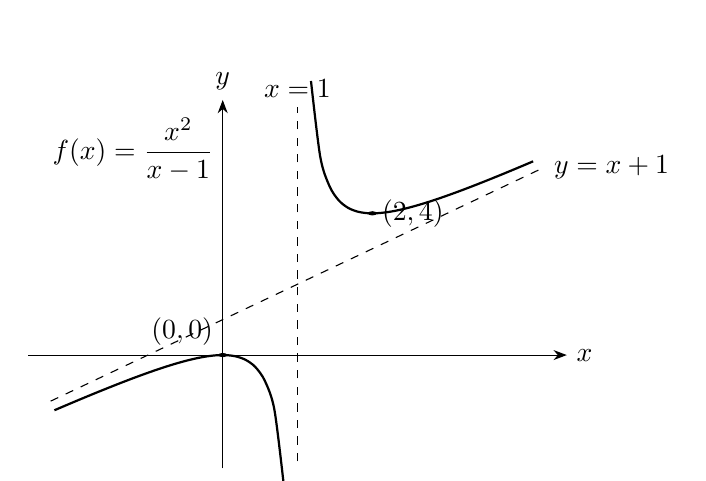
\begin{tikzpicture}[xscale=0.95,yscale=0.45,>=Stealth]
  \draw[->] (-2.6,0)--(4.6,0) node[right] {$x$};
  \draw[->] (0,-3.2)--(0,7.2) node[above] {$y$};
  \draw[dashed] (1,-3.0)--(1,7.0) node[above] {$x=1$};
  \draw[dashed] (-2.3,-1.3)--(4.3,5.3) node[right] {$y=x+1$};
  \draw[domain=-2.25:0.82,smooth,variable=\x,thick]
    plot ({\x},{\x+1+1/(\x-1)});
  \draw[domain=1.18:4.15,smooth,variable=\x,thick]
    plot ({\x},{\x+1+1/(\x-1)});
  \fill (0,0) circle (1.7pt) node[above left] {$(0,0)$};
  \fill (2,4) circle (1.7pt) node[right] {$(2,4)$};
  \node at (-1.2,5.8) {$f(x)=\dfrac{x^2}{x-1}$};
\end{tikzpicture}
\end{center}

\subsection{Taylor 公式}

\begin{theorem}[Taylor 公式：Lagrange 余项]
若 $f$ 在含 $x_0$ 与 $x$ 的区间上有 $n+1$ 阶连续导数，则存在介于 $x_0$ 与 $x$ 之间的 $\xi$，使得
\[
f(x)=\sum_{k=0}^{n}\frac{f^{(k)}(x_0)}{k!}(x-x_0)^k
+\frac{f^{(n+1)}(\xi)}{(n+1)!}(x-x_0)^{n+1}.
\]
\end{theorem}
\begin{proofdetail}
记
\[
P_n(t)=\sum_{k=0}^{n}\frac{f^{(k)}(x_0)}{k!}(t-x_0)^k.
\]
固定 $x\neq x_0$，令
\[
R=f(x)-P_n(x),\qquad
M=\frac{R}{(x-x_0)^{n+1}}.
\]
构造
\[
F(t)=f(t)-P_n(t)-M(t-x_0)^{n+1}.
\]
由 $P_n$ 的构造可知
\[
F(x_0)=F'(x_0)=\cdots=F^{(n)}(x_0)=0,
\]
且由 $M$ 的定义，$F(x)=0$. 对 $F$ 在以 $x_0,x$ 为端点的区间反复使用 Rolle 定理：由 $F(x_0)=F(x)=0$，存在一点使 $F'=0$；又 $F'(x_0)=0$，可在相应子区间再次使用 Rolle 定理，逐次得到存在 $\xi$ 介于 $x_0$ 与 $x$ 之间，使
\[
F^{(n+1)}(\xi)=0.
\]
而
\[
F^{(n+1)}(t)=f^{(n+1)}(t)-M(n+1)!.
\]
故
\[
M=\frac{f^{(n+1)}(\xi)}{(n+1)!}.
\]
代回 $R=M(x-x_0)^{n+1}$，得 Taylor 公式.
\end{proofdetail}

\begin{example}[Maclaurin 公式]
写出 $\ee^x,\sin x,\ln(1+x)$ 在 $0$ 处到常用阶数的展开.
\end{example}
\begin{solution}
\[
\ee^x=1+x+\frac{x^2}{2!}+\cdots+\frac{x^n}{n!}+o(x^n).
\]
\[
\sin x=x-\frac{x^3}{3!}+\frac{x^5}{5!}+\cdots+(-1)^m\frac{x^{2m+1}}{(2m+1)!}+o(x^{2m+1}).
\]
\[
\ln(1+x)=x-\frac{x^2}{2}+\frac{x^3}{3}-\cdots+(-1)^{n-1}\frac{x^n}{n}+o(x^n).
\]
这些公式可由 Taylor 公式和各阶导数在 $0$ 处的值推出.
\end{solution}

\begin{example}[极限]
求 $\displaystyle\lim_{x\to0}\frac{\cos x-1+\frac{x^2}{2}}{x^4}$.
\end{example}
\begin{solution}
由 Taylor 展开
\[
\cos x=1-\frac{x^2}{2}+\frac{x^4}{24}+o(x^4).
\]
故分子为
\[
\left(1-\frac{x^2}{2}+\frac{x^4}{24}+o(x^4)\right)-1+\frac{x^2}{2}
=\frac{x^4}{24}+o(x^4).
\]
因此极限为 $1/24$.
\end{solution}

\begin{example}[用 Taylor 判别极值]
设 $f'(x_0)=f''(x_0)=0$，$f^{(3)}(x_0)\neq0$. 证明 $x_0$ 不是极值点.
\end{example}
\begin{solution}
由 Taylor 公式，
\[
f(x)=f(x_0)+\frac{f^{(3)}(x_0)}{3!}(x-x_0)^3+o((x-x_0)^3).
\]
记 $A=f^{(3)}(x_0)/6\neq0$. 则
\[
f(x)-f(x_0)=(x-x_0)^3[A+o(1)].
\]
当 $x$ 足够接近 $x_0$ 时，$A+o(1)$ 与 $A$ 同号. 而 $(x-x_0)^3$ 在 $x_0$ 两侧异号，所以 $f(x)-f(x_0)$ 在两侧异号. 因此 $f(x_0)$ 既不是局部极大值，也不是局部极小值.
\end{solution}

\subsection{课后习题（二）：凸性、渐近线与 Taylor 公式}
\begin{enumerate}[label=\textbf{练习\arabic*.},leftmargin=2.2em]
\item 讨论 $y=x^4-2x^2$ 的凸性与拐点.
\item 求 $f(x)=\frac{x^2+1}{x-1}$ 的垂直渐近线与斜渐近线.
\item 用 Taylor 公式求下列极限或近似：
\[
\lim_{x\to0}\frac{\ln(1+x)-x+\frac{x^2}{2}}{x^3},\quad
\lim_{x\to0}\frac{\ee^{x^2}-1}{1-\cos x},\quad
\sqrt[3]{8.12}.
\]
\end{enumerate}

\subsection{参考解答（二）}
\begin{enumerate}[label=\textbf{练习\arabic*.},leftmargin=2.2em]
\item
\[
y''=12x^2-4=4(3x^2-1).
\]
当 $|x|<1/\sqrt3$ 时 $y''<0$，曲线上凸；当 $|x|>1/\sqrt3$ 时 $y''>0$，曲线下凸. 拐点为
\[
\left(\pm\frac1{\sqrt3},\,\frac19-\frac23\right)=\left(\pm\frac1{\sqrt3},-\frac59\right).
\]
\item $x=1$ 是垂直渐近线. 作除法：
\[
\frac{x^2+1}{x-1}=x+1+\frac2{x-1},
\]
故斜渐近线为 $y=x+1$.
\item
\[
\ln(1+x)=x-\frac{x^2}{2}+\frac{x^3}{3}+o(x^3),
\]
故第一个极限为 $\frac13$. 又
\[
\ee^{x^2}-1=x^2+o(x^2),\qquad 1-\cos x=\frac{x^2}{2}+o(x^2),
\]
第二个极限为 $2$. 对 $\sqrt[3]{8.12}$，取 $f(x)=x^{1/3}$，在 $x=8$ 处线性化：
\[
\sqrt[3]{8.12}\approx2+\frac{1}{3\cdot 8^{2/3}}\cdot0.12=2+\frac{0.12}{12}=2.01.
\]
\end{enumerate}

\clearpage
\renewcommand{\refname}{References}
\addcontentsline{toc}{section}{References}
\begin{thebibliography}{99}
\bibitem{JJ} 龚德恩. 经济数学基础：第一分册，微积分. 四川人民出版社. 2016.
\bibitem{TJ} 同济大学数学系. 高等数学. 高等教育出版社.
\bibitem{CJX} 陈纪修，於崇华，金路. 数学分析. 高等教育出版社.
\bibitem{Stewart} Stewart, J. \emph{Calculus: Early Transcendentals}. Cengage Learning.
\end{thebibliography}

\end{document}
